\documentclass[a4paper,10pt]{article}
% define the title
\usepackage{graphicx}
\usepackage{graphicx}
\usepackage{array}
\usepackage{amsmath}
\usepackage{natbib}
\usepackage{CJK}
\usepackage[dvipdfm,
            pdfstartview=FitH,
            CJKbookmarks=true,
            bookmarksnumbered=true,
            bookmarksopen=true,
            colorlinks, %注释掉此项则交叉引用为彩色边框(将colorlinks和pdfborder同时注释掉)
            pdfborder=001, %注释掉此项则交叉引用为彩色边框
            linkcolor=blue,
            anchorcolor=blue,
            citecolor=blue
            ]{hyperref}
%===================== 重定义字体、字号命令 =====================%
\newcommand{\song}{\CJKfamily{song}}    % 宋体   (Windows自带simsun.ttf)
\newcommand{\fs}{\CJKfamily{fs}}        % 仿宋体 (Windows自带simfs.ttf)
\newcommand{\kai}{\CJKfamily{kai}}      % 楷体   (Windows自带simkai.ttf)
\newcommand{\hei}{\CJKfamily{hei}}      % 黑体   (Windows自带simhei.ttf)
\newcommand{\li}{\CJKfamily{li}}        % 隶书   (Windows自带simli.ttf)
\newcommand{\you}{\CJKfamily{you}}      % 幼圆   (Windows自带simyou.ttf)
%
\newcommand{\chaoda}{\fontsize{55pt}{\baselineskip}\selectfont}
\newcommand{\chuhao}{\fontsize{42pt}{\baselineskip}\selectfont}     % 字号设置
\newcommand{\xiaochuhao}{\fontsize{36pt}{\baselineskip}\selectfont} % 字号设置
\newcommand{\yihao}{\fontsize{28pt}{\baselineskip}\selectfont}      % 字号设置
\newcommand{\erhao}{\fontsize{21pt}{\baselineskip}\selectfont}      % 字号设置
\newcommand{\xiaoerhao}{\fontsize{18pt}{\baselineskip}\selectfont}  % 字号设置
\newcommand{\sanhao}{\fontsize{15.75pt}{\baselineskip}\selectfont}  % 字号设置
\newcommand{\xiaosanhao}{\fontsize{15pt}{\baselineskip}\selectfont} % 字号设置
\newcommand{\sihao}{\fontsize{14pt}{\baselineskip}\selectfont}      % 字号设置
\newcommand{\xiaosihao}{\fontsize{12pt}{14pt}\selectfont}           % 字号设置
\newcommand{\wuhao}{\fontsize{10.5pt}{12.6pt}\selectfont}           % 字号设置
\newcommand{\xiaowuhao}{\fontsize{9pt}{11pt}{\baselineskip}\selectfont}   % 字号设置
\newcommand{\liuhao}{\fontsize{7.875pt}{\baselineskip}\selectfont}  % 字号设置
\newcommand{\qihao}{\fontsize{5.25pt}{\baselineskip}\selectfont}    % 字号设置
%=============================================================================%
\renewcommand\listfigurename{图 目 录}
\renewcommand\listtablename{表 目 录}
\renewcommand\figurename{图}
\renewcommand\tablename{表}
\begin{CJK}{GBK}{st}\end{CJK}

%====================定义图,公式标编号等格式=============
\numberwithin{figure}{section} \numberwithin{table}{section}
\numberwithin{equation}{section}
\renewcommand{\theequation}{\thesection.\arabic{equation}}
\renewcommand{\thefigure}{\arabic{section}-\arabic{figure}}
\renewcommand{\thetable}{\arabic{section}-\arabic{table}}
%==========================================================
%==================================================================
%==================================================================
%==================================================================
%==================================================================
%==================================================================
%==================================================================
\begin{document}
\begin{CJK}{UTF8}{gbsn}
\author{陈林}
\title{Codger一种面向对象语言的设计和解析器的设计与实现}
\date{2012-4-5}
\maketitle
\newpage
\tableofcontents
\newpage
%

\section{简介}
\subsection{Codger简介}
Codger是一门面向对象,直译式的动态程序设计语言,在Codger中一切皆为对象:整数,字符串,函数,类象,模块等等都被视为对象。所有的对象都是在运行时,才能确定它们的类型,在编写程序时,可以将任意类型的对象赋值给同一个变量,变量在使用和赋值前,不需要预先申明。同样不用申明变量的类型。

Codger提供了丰富的基本数据类型用于简化程序的编写,每次运行程序时不需要对程序进行预编译,直接运行即可。因为Codger支持式的特性,它可以交互式编程,即输入语句后,可以立即得到结果,然后再根据结果输入下一条语句。

和大多数高级语言一样,使用Codger编程时,不需要考虑内存分配问题,创建的对象不需要手动的释放,Codger有自己的垃圾收集器,当一个对象成为垃圾时,它们会被垃圾收集器回收。



\subsection{解析器简介}
解析器用于解析并运行Codger源程序,当Codger源文件被解析时,它的处理过程如图\ref{fig:fileprocess}。解析器分成两部分:解析器前端和解析器后端。解析器前端负责检查源程序中的词法、语法错误,生成与源程序等价的抽象语法树,并根据抽象语法树生成模块对象,模块对象是源程序的一种等价表示,它包含了源程中出现的所有常量和标识符以及源程序被转换后的字节码等信息。解析器后端也被称作为虚拟机,它负责字节码的运行,异常处理以及内存管理等。


\begin{figure}
\centering
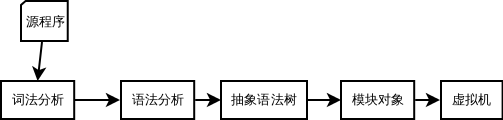
\includegraphics[scale=0.8]{file_process.png}
\label{fig:fileprocess}
\caption{解析器工作流程} 
\end{figure}



%\section{词法}
codger源程序由一系列具有独立意义的基本语法单位--单词组成,单词是最小的词法单位,它们不能分割。单词分为8类:关键字,运算符,特殊符号,整数,长整数,浮点数,字符串,标识符,空白符,注释,其中空白符与注释属于无用单词,当被扫描器识别到时,会立刻被弃。

解析器中的语法识别模块用于对codger源程序进行词法分析,从输入字符流中扫描出由字符序列组成的单词。并把识别出的单词交给后面的语法分析模块进一步处理,并在识别过程中检测是否存在非法的单词。
\subsection{关键字}
codger中关键字具有专门的意义与用途,它们不能被当作一般的标识符来使用,这些关键字有:
\begin{quote}
\begin{verbatim}
and, as, attr, break, catch, class, continue, export,
do, elif, else, end, false, finally, for, from, func, 
if, import, in, inherit, new, not, or, print, private, 
protected, public, return, static, then, to, true,
try, while。
\end{verbatim}
\end{quote}
\subsection{标识符}
标识符用于定义变量,函数,类,方法等所使用的名称,解析器没有限定标识符的长度,但在定义标识符时,需要遵守一定的规则:以字母或者下画线开头,后面可以接零个或多个字母、数字、下画线,并且区会字母的大写与小写。用文法表示为:
\begin{quote}
\begin{verbatim}
identifier =(letter|"_"|)(letter|digit|"_")*
digit ="0".."9"
letter =lowercase|uppercase
lowercase ="a".."z"
uppercase ="A".."Z"
\end{verbatim}
\end{quote}
\subsection{特殊符号与运算符}
在codger中,运算符用于指定一种运算方式,特殊符号用于分隔不同的语句或者用于指定某些特定意义的用途。它们有:
\begin{quote}
\begin{verbatim}
 (   )   [   ]   .   ,  +   -   ~   *  ;
 /   %  <<   >>   <   >   <=   >=  ==  {  }
 !=   &   ^   | =   +=   -=   *=   /=  ->
 %=   &=   ^=   |=   >>=   <<=  换行符
\end{verbatim}
\end{quote}
\subsection{整数}
整数是一种与机器平台相关的数据类型,在32位机上,其表示范围为 $-2^{31}$ 到 $2^{31}-1$。而在64位机上,其表示范围为$-2^{63}$ 到 $2^{63}-1$ 。整数的表示范围有限,在设计程序时需要考虑运算结果溢出的情况。整数可以在codger源程序中显示的定义,整数又被分为二进制整数,八进制整数,十进制整数,十六进制整数。二进制整数以0b或者0B开头,后面紧接着一个或多个0或1;八进制整数以0或者0o、0O开头,后面紧接数字一个或多个0-7;十进制整数以1-9开头,后面紧接数字零个或多个0-9,或者是只有一位十进制整数0;十六进制整数以0x或都0X开头,后面紧接一个或者多个数字0-9、a-f、A-F。用文法表示为:
\begin{quote}
\begin{verbatim}
integer =decimalinteger|octinteger|hexinteger|bininteger
decimalinteger = nonzerodigit digit* | "0"
octinteger = "0" ("o" | "O") octdigit+ | "0" octdigit+
hexinteger = "0" ("x" | "X") hexdigit+
bininteger = "0" ("b" | "B") bindigit+
nonzerodigit = "1"..."9"
octdigit = "0"..."7"
bindigit = "0" | "1"
hexdigit:= digit | "a"..."f" | "A"..."F"
\end{verbatim}
\end{quote}

\subsection{长整数}
整数表示范围有限,在进行大数据运算时受到限制,Codger 提贡长整数用于解决这种问题。长整数是一种与机器无关的数据类型,可以进行任意大小的数据运算,不用去考虑数据溢出问题,但是前提是你的计算机有中够大的内存空间,来保存这些数据。 长整数可以在源程序中显示的定义,定义方法同整数一样,只有在后面多了一位字符L或者是l。用文法表示为:
\begin{quote}
 \begin{verbatim}
  longinteger = integer ("l" | "L")
 \end{verbatim}
\end{quote}

\subsection{浮点数}
在codger中采用的是32位浮点数,其数值范围约为:$-3.4*10^{-38}$ 到 $-3.4*10^{38}$ 。浮点数由三个部分组成:整数部分,浮点部分,指数部分。浮点数可以在源程序中显示定义,定义时整数部分与指数部分可以省去。用文法表示浮点数为:
\begin{quote}
 \begin{verbatim}
floatnumber = pointfloat | exponentfloat
pointfloat = [intpart] "." digit+
exponentfloat = (intpart | pointfloat) exponent
intpart = digit+
exponent = ("e" | "E") ["+" | "-"] digit+
 \end{verbatim}
\end{quote}
\subsection{字符串}
字符串可以在源程序中显示定义,使用规则为:以双引号开头和双引号结尾,中间可以是除 \verb \ 和换行符以处的任意字符,其中\verb \ 用于转义其它特殊字符,如果想要以多行的形式书写字符串,需要在每一行的未尾加上\verb \ 。用文法表示为:
\begin{quote}
 \begin{verbatim}
string =`"'stringitem*`"'
stringitem = <any source character except "\" 
				or newline or the quote> |"\"esc_item
esc_item =<any source character >
 \end{verbatim}
\end{quote}
\subsection{注释}
在Codger注释以\#号开头,直到这一行结果,解析器解析源程序,注释中的所有内容都分被忽略掉。用文法表示为:
\begin{quote}
 \begin{verbatim}
comment ="#" cm_item* newline
cm_item =<any source character except newline>
 \end{verbatim}
\end{quote}
\subsection{空白符}
Codger中的空白符由一个或都多个空格或者是制表符组成,程序中的空白符用于区分开不同的单词,或者使源程序的可读性更强。当解析器识别到空白符时,不会对它做任何的处理,只是简单的将它抛弃。用文法表示为:
\begin{quote}
 \begin{verbatim}
white_space =ws_item+
ws_item = space | tab 
 \end{verbatim}
\end{quote}


\newpage
\section{词法识别算法}
在前面一部分给出了在codger中所有的单词,以及描述单词结构的bnf文法,这些文法都是正则文法。正则文法与有限状态机具有等价性,它们之间可以相互转换\footnote{等价性的证明以及转换的方法可以参考``形式语言与自动机理论''}。而词法识别算法通常是通过构造有限状态机的方法来识别源程序中的不同类型的单词,状态机可以使用类似于lex的词法分析软件自动生成,这种方法处理起来简单,只需要遵守词法分析软件的使用规则即可,或者程序员可以通过手工来构造状态机。手工构造相比词法分析软件相比优点在于:
\begin{enumerate}
 \item 词法分析软件有固定处理框架,不能随意改变,限定了程序的灵活性。手工构造则没有这种限制。
 \item 词法分析软件根据一定算法生成有限状态机,其中有许多重复的或者是多余的状态都可以被优化掉。
\end{enumerate}
但手工构造如果处理不好,可能会随着正则语言规模的增大,复杂度也跟着增加,最终可以超出人脑可能处理的限度。下面介绍一种在codger词法分析模块中使用的一种算法--状态链。
\subsection{状态链简介}
在codger解析器的早期版本中,采用状态矩阵\footnote{大多数编译原理书本都会介绍状态矩阵算法,这里不对其进行详细说明}的方法来识别源程序中的单词。但由于状态矩阵算法会随着正则文法规模的增大,复杂度也跟着增加,每次当需要变更每个单词的结构时,都需要更改一大堆数据,使解析器的维护的扩展都变得非常困难,而且极容易出错。最后不得不放弃状态矩阵,而寻找新的方法。

状态链识别法是在codger解析器开发过程中总结出的一种非常实用和高效的算法,之所以命名为状态链,因为状态链算法处理的最多的是状态与状态之间的链接。状态链算法优点再于:
\begin{enumerate}
 \item 随着正则文法规模的变大,其复杂度一般情况下不会增加。
 \item 状态链是一种分治算法,它先通过为每一个不同类型的单词构造子状态机,然后再通过合并算法把子状态机合并在一起,合并时,不需要更改子状态机中的数据和状态,只需增加新的状态链接到子状态机中已有的状态。
 \item 状态机中的每个状态只需要处理它所接受输入事件类型,以及在该输入事件类型下的后继状态,而不用去了解状态机的整体结构。当状态机的结构发生变化时,很多状态都可以直接得到重用,使解析器的维护和扩展变得非常容易。
\end{enumerate}
\subsection{状态的结构}
状态链算法中,许多的状态链接在一起构成一个有限状态机,在每个状态中都会保存与该状态相关的基本信息,这些信息有:
\begin{enumerate}
 \item 状态是否为终态,如果是终态,同时也会保存该状态所属单词的类型,单词类型用于后面的语法分析。
 \item 字符映射数组:字符射数组长度为256,codger源程序是由字符序列组成,每当解析器从源程序中读出一个字符时,该字符的值的范围为:0到255,然后从字符映射数组获得输入事件类型。
 \item 状态能接受的输入事件类型,以及在该输入类型下所转换到的后继状态。
\end{enumerate}
用程序来描述为(attr表示属性定义):
\begin{quote}
 \begin{verbatim}
class State
    attr finally        #是否为终态
    attr token          #单词的类型
    attr input_map[256] #字符映射数组
    attr targets[]      #后继状态
end
 \end{verbatim}
\end{quote}
例如:假设状态a为不为终态,在字符`0'到`9'下转移到状态b,在`a'到`f'下转移到状态c,在其它状态下,转换到错误状态。为状态a构造状态数据为:
\begin{quote}
 \begin{verbatim}
State a
    finally=false
    token="unkown"
    input_map=[0,0,0,0,0,0,0,0,0,0,0,0,0,0,0,0
               0,0,0,0,0,0,0,0,0,0,0,0,0,0,0,0
               0,0,0,0,0,0,0,0,0,0,0,0,0,0,0,0
               1,1,1,1,1,1,1,1,1,1,0,0,0,0,0,0
               0,0,0,0,0,0,0,0,0,0,0,0,0,0,0,0
               0,0,0,0,0,0,0,0,0,0,0,0,0,0,0,0
               0,2,2,2,2,2,0,0,0,0,0,0,0,0,0,0
               0,0,0,0,0,0,0,0,0,0,0,0,0,0,0,0
                       .........
               0,0,0,0,0,0,0,0,0,0,0,0,0,0,0,0]
    targets=[err,b,c]
end  
 \end{verbatim}
\end{quote}

其中在input\_map中的省略号为112个0,状态a总共能接受三种输入事件类型,由于数组脚标从零开始,所以三种输入事件类型分别称为输入事件0,输入事件1,输入事件2
\begin{enumerate}
 \item 输人字符`0'到`9'会被映射为第1种输入事件类型,状态a在该输入类型下会转移到后继状态b,状态b保存在targets中的脚标为1的位置
 \item 输入字符`a'到`f'会被映射为第2种输入事件类型,状态a在该输入类型下会转移到后继状态c,状态c保存在targets中的脚标为2的位置
 \item 除`0'到`9'和`a'到`f'以外的所有字符会被映射到第0种输入事件类型,状态a在该输类型下会转移到后断状态err,状态err保存在targets中的脚标为0的位置。状态err是一个内置状态,用于表示源程于中单词存在错误。
\end{enumerate}

input\_map是一个256位的数组,数组元素类型为unsigned char, unsigned char占用一个字节,即一个input\_map需要256字节。但并不是每个状态都需要独自拥有一个字符映射数组。在很多情况下,许多状态的输入事件类型相似,或者是完全相同,它们可以建立一个公有的字符映射数组,用于共享,以提高内存的利用率。例如状态a在符号`c'到`z'转换到状态c,状态b在字符`a'到`f'能转换到状态c,虽然状态a与状态b能接受的输入事件类型不同,但是可能通过合并状态a与状态b输入事件,让它们共享一个字符映射数组。合并方法为:提取出字符`c'到z'与字符`a'到`f'两个序列范围的交集部分为:字符`c'到`f',即现在的有四种输入类型
\begin{quote}
1) 类型0, 字符`a'到`b' \\
2) 类型1, 字符`c'到`f' \\
3) 类型2, 字符`g'到`z' \\
4) 类型3, 除前面字符以外的所有字符。 
\end{quote}
以前状态a是在字符`c'到`z'转换到状态c,现在改为在字符`a'到`b'与字符`c' 到 `f'的情况下转换到c;以前状态b是在字符`c'到`z'转换到状态c,现在改为在字符`c'到`f'与字符`g'到`z'的情况下转移到状态c。在合并字符映射数组后,a的后继状态数组改为[c,c,err,err],b的后继状态数组为[err,c,c,err]。

Codger解析器的词法识别模块大约有90多个状态和10字符映射组成,基本上每种单词类型的所有状态共享一个状态映射数组。词法识别模块所占用的内存大约在4k左右。
\subsection{识别算法}
Codger的词法识别算法是基于有限状态机,在词法识别模块保存了一个完整的,能识别到codger语言中所有单词的有限状态机。当解析器解析codger源程序时,采用最大识别的方法,下面为识别一个单词大概步骤:
\begin{enumerate}
 \item 置当前状态置为有限状态机的开始状态
 \item 从输入字符流中读出一个字符
 \item 根据当前状态与输入字符确定下一个状态,并置当前状态为下一状态
 \item 处理当前状态,当前状态的类型有三种情况:普通状态,终态,错误状态
 \begin{enumerate}
 	\item 普通状态:跳转的步聚2
 	\item 终态:则记录下该状态与输入字符流的位置。并且跳转到步聚2
 	\item 错误状态:查看以前是否到达过终态,如果是则选择最近一次到达的终态,把多识别的字符返回给输入字符流,返回该单词的类型。如果没有到达过终态,则表明源程序中存在词法错误,返回出错信息。
 \end{enumerate}
\end{enumerate}
用代码来描述为:
\begin{quote}
\begin{verbatim}
GetToken(f)                    
    cur_state=begin_state      #设置当前状态为开始状态
    finally_state=Nil          #以及初始化程序数据
    file_pos=Nil
    while true 
        c=f.getchar()                 #从文件读出一个字符
        cur_state=cur_state.next(c)   #获取下一状态
        if cur_state==err         
            if finally_state!= Nil    #以前到达过终态
                f.set_read_pos(file_pos)  
                return finally_state.token  
            else                      #以前没有到达过终态
                return  ERR_TOKEN  
            end
        elif cur_state.finally        #如果为终态
            finally_state=cur_state   #保存该状态
            file_pos=f.get_read_pos   #保存文件的读位置
        end
    end
end 
\end{verbatim}
\begin{center}
 代码4.3.1
\end{center}
其中State.next的代码如下:
\end{quote}
\begin{quote}
\begin{verbatim}
State.next(c)
    input_type=State.input_map[c]    #获取输入类型
    return State.targets[input_type] #找到后继状态并返回
end 
\end{verbatim}
\end{quote}

涉及到识别到错误状态时,读位置的回退操作,回退的平均位移为2,所以代码4.3.1的时间算杂度与基本上与源文件的字符长度成正比。
  
\subsection{状态机的合并}
在前面介绍过,状态链算法是一种分治的算法,其主要思想为先为每个不同类型的单词构造子状态机,然后通过合并算法把子状态机合并成为一个大的综合性的状态机。假设现在有两个状态机:
\begin{quote}
1) 状态机A用于识别正则式[0-7]+abf所表示的语言,如图\ref{fig:state_a}\\
2) 状态机B用于识别正则式[4-9]+acd所表示的语言,如图\ref{fig:state_b}
\end{quote}
\begin{figure}
 \centering
 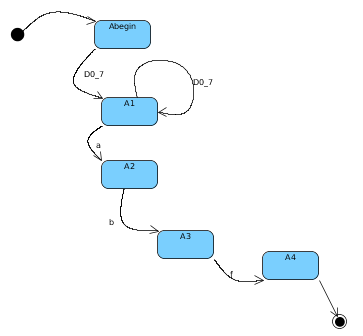
\includegraphics[scale=1]{s_a.png}
 \caption{状态机A}
 \label{fig:state_a}
\end{figure}
为了减少字符映射数组的使用,让状态机A的所有状态共享一个状态映射数组,这样一来,对于每个状态来说就有5种输入类型,同样也就有5个后继状态:
\begin{quote}
1) 数字0到7,命名为 D0\_7  \\
2) 字符a,命名为 S\_a  \\
3) 字符b,命名为 S\_b \\
4) 字符f,命名为 S\_f \\
5) 除以上字符以外的所有字符,命名为 Other
\end{quote}
例如状态机A中的状态A1的后继状态为:[A1,A2,err,err,err] 

同样对状态机B中的所有状态也让它们共享一个状态映射数组,则对于每个状态来说,输入类型有5种,5个后继状态:
\begin{quote}
1) 数字4到9,命名为 D4\_9 \\
2) 字符a,命名为 S\_a \\
3) 字符c,命名为 S\_c \\
4) 字符d, 命名为 S\_d \\
5) 除以上字符以外的所有字符,命名为 Other
\end{quote}
\begin{figure}
 \centering
 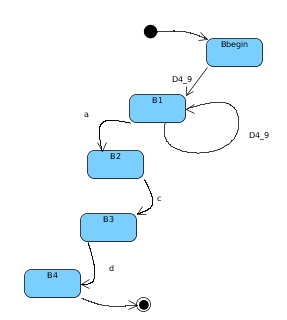
\includegraphics[scale=1]{s_b.png}
 \caption{状态机B}
 \label{fig:state_b}
\end{figure}
合并过程如下:
\begin{description}
\item[第一步:]合并状态机A与状态B的输入类型,找出相交输入类型,提取出它们的公有子集,输入类型合并的有9种:
\begin{quote}
1) 数字0到3, 命名为 D0\_3 \\
2) 数字4到7, 命名为 D4\_7 \\
3) 数字8到9, 命名为 D8\_9 \\
4) 字符a,  命名为 S\_a \\
5) 字符b,  命名为 S\_b \\
6) 字符c,  命名为 S\_c \\
7) 字符d,  命名为 S\_d \\
8) 字符f,  命名为 S\_f \\
9) 除以上字符以外的所有字符, 命名为 Other
\end{quote}
其中状态机A中的输入类型D0\_7被分解成为了输入类型D0\_3和D4\_7;状态机中的输入类型D4\_9被分解成了输入类型D4\_7和D8\_9
\item[第二步:]状态机A的开始状态为Abegin,状态机B的开始状态为Bbegin,创建一个状态复合状态 \{Abeign ,Bbegin\}, 把该复合状态命名为Cbegin,并且标记Cbegin。其中复合状态的定义为:复合状态中的任意一个状态能在某种输入类型下发生状态转移,该复合状态也能在该输入类型下发生状态转移,并且后继状态相同。
\item[第三步:]找出一个被标记的复合状态,现在只有Cbeign被标记,所以取出 Cbegin,然后取消标记 Cbeign,并确定Cbegin的后继状态,Cbeign 为 \{Abegin ,Bbegin\} 的复合状态:\\
因为:
\begin{quote}
\begin{verbatim}
f(Abegin,D0_7)->A1
f(Bbegin,D4_9)->B1
\end{verbatim}
\end{quote}
推出:
\begin{quote}
\begin{verbatim}
f(Cbegin,D0_3)->A1
f(Cbegin,D4_7)->{A1,B1}
f(Cbegin,D8_9)->B1
\end{verbatim}
\end{quote}
CBegin的转换情况如下表\footnote{空白的地方表示状态CBegin在该输入类型转移到err}:

\begin{tabular}[c]{c|c|c|c|c|c|c|c|c|c}
状态\slash输入&	D0\_3&D4\_7&D8\_9&S\_a&S\_b&S\_c&S\_d&S\_f&Other \\
\hline
CBegin&A1&A1,B1&B1&&&&&&\\
\hline
\end{tabular}

在确定后继状态,需要处理的其中的复合状态,Cbeign在输入事件D4\_7下转移到复合状\{A1,B1\},该复合状态以前并没出现过,创建复合状态\{A1,B1\},把该状态命名为C1,标记C1。
\item[第四步:] 检测现在是否存在被标记的复合状态,如果存在,跳转到第三步。如果没有,则状态机的合并完成。现在状态C1被标记,将其取出,取消标记C1,C1 为 \{A1,B1\} 的复合状态:\\
因为:
\begin{quote}
\begin{verbatim}
f(A1,D0_7)->A1
f(A1,S_a)->A2
f(B1,D4_9)->B1
f(B1,S_a)->B2
\end{verbatim}
\end{quote}
推出:
\begin{quote}
\begin{verbatim}
f(C1,D0_3)->A1
f(C1,D4_7)->{A1,B1}
f(C1,D8_9)->B1
f(C1,S_a)->{A2,B2}
\end{verbatim}
\end{quote}

C1的状态转移如下表:

\begin{tabular}[c]{c|c|c|c|c|c|c|c|c|c}
状态\slash输入&	D0\_3&D4\_7&D8\_9&S\_a&S\_b&S\_c&S\_d&S\_f&Other \\
\hline
C1&A1&A1,B1&B1&A2,B2&&&&& \\
\hline
\end{tabular}

C1的后继中状态中有两个复合状态,其中复合状态\{A1,B1\}在以前已经被创建过,所以不对其进行处理。复合状态\{A2,B2\}以前没有出现过,则创建它,并且标记,把它命名为C2。

现在还存在标记的复合状态C2,所以继续按照每二步的方法来处理,取出C2,取消标记,C2为 \{A2, B2\} 的复合状态: \\
因为:
\begin{quote}
\begin{verbatim}
f(A2,S_b)=A3
f(B2,S_c)=B3
\end{verbatim}
\end{quote}
推出:
\begin{quote}
\begin{verbatim}
f(C2,S_b)=A3
f(C2,S_c)=B3
\end{verbatim}
\end{quote}

C2的状态转移如下表:

\begin{tabular}[c]{c|c|c|c|c|c|c|c|c|c}
状态\slash输入&	D0\_3&D4\_7&D8\_9&S\_a&S\_b&S\_c&S\_d&S\_f&Other \\
\hline
C2&&&&&A3&B3&&& \\
\hline
\end{tabular}
\end{description}

现在以经没有被标记过的状态,表示状态机的整个合并过程完成,合并后创建了3个新状态:CBegin, C1, C2。每个状态接受的输入类型有9个,但可以对其进行优化,因为三个状态在输入类型 S\_d, S\_f ,Other 下都转移到err,可以把它们合并到输入类型Other中,即最终的输入类型7个:
\begin{quote}
1) 数字0到3, 命名为 D0\_3 \\
2) 数字4到7, 命名为 D4\_7 \\
3) 数字8到9, 命名为 D8\_9 \\
4) 字符a,  命名为 S\_a \\
5) 字符b,  命名为 S\_b \\
6) 字符c,  命名为 S\_c \\
7) 除以上字符以外的所有字符, 命名为 Other
\end{quote}
合并后的状态图为:图\ref{fig:state_c}, 每个状态后继状态如下:
\begin{quote}
1) CBegin后继状态为:[A1,C1,B1,err,err,err,err]  \\
2) C1后继状态为:[A1,C1,B1,C2,err,err,err] \\
3) C2后继状态为:[err,err,err,err,A3,B3,err] 
\end{quote}
\begin{figure}
\centering
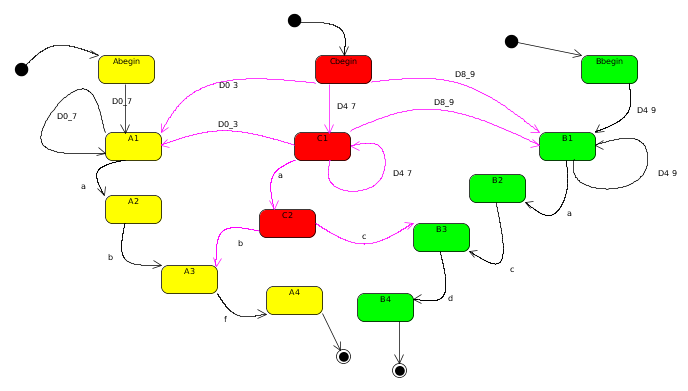
\includegraphics[scale=0.8,angle=90]{s_c.png}
\caption{状态机A与状态机B后并后}
\label{fig:state_c}
\end{figure}
状态机A与状态B的合并过程中,并不会改变状态A与状态机B的任何一个状态的信息,合并后创建了3个的新状态。新状态通过后继状态链接到子状态机A与子状态机B中的状态。把识别算法中的开始状态改为Cbegin,就可以对正则式[0-7]+abf和[4-9]+acd表示的语言进行识别。因为子状态的数据没有被改变,当只需要识别正则式[0-7]+abf所表示的语言时,同样也只需要把识别算法中的开始状态改变Abegin即可,这种特性使模块的调试变得很简单,可以先测试子状态机A和子状态机B是否正确,然后再测试合并后的状态机是否正确。

在Codger词法中有9个不同类型的单词,关键字的识别是通用先识别出标识符,然后再判断标识符是否属于关键字。子状态机有8个,识别每种单词类型子状态机的开始符号所接受的输入事件类型之间的交集很少,例如:注释以\#号开头,整数和以数字开头,浮点数以数字和点号开头,字符串以双引号开头,标识符以字母开头,在合并的时,涉及到的复合状态很少,最复杂的合并属于浮点数与整数的合并,但合并后也只创建了4个新的状态。


%\section{数据类型}
\subsection{对象}
Codger语言的整体的设计思想为:一切皆是对象。整数,浮点数,字符串等基本的数据类型是对象,函数是对象,甚至类也是对象\ldots{} 因为这种特性,可以在源程序中使用类似于下面的语句:
\begin{quote}
\begin{verbatim}
print 1.add(3)  #输出1+3的值
print "Codger".length() #输出字符串"Codger"的长度
\end{verbatim}
\end{quote}
对象Object是所有对象的父类,也就是说所有对象直接或者间接的继承对象Object。每个对象所携带的信息分为两部分:1)对象的类型信息,用于标识该对象的类型,所有同类型的对象共享对象的类型信息,类型信息里面保存了对象的所属类型,对象使用私有数据的方法,对象与其它对象交互的方式等。类型信息在对象创建时绑定到对象上。2)对象的私有数据,不同的对象有不同的私有数据,不同类型的对象对私有数据的使用方法也不同,例如整数对象的私有数据部分用于保存数值,字符串对象的私有数据用于保存字符序列。
\subsection{变量}
Codger是一门动态类型语言,所有对象的类型都是在运行时才能确定,变量在使用时不需要预先申明,也不需要申明变量的类型,可以不同的时刻给变量赋值不同类型的对象,例如下面的语句:
\begin{quote}
\begin{verbatim}
a=2          #把整数对象2赋值给变量a
a="Codger"   #把字符串对象"Codger"赋值变量a 
\end{verbatim}
\end{quote}
当对一个变量赋值时,变量中会保存到该对象的引用,如果访问一个未引用对象的变量时,虚拟机会抛出变量未定义的异常。当把一个变量赋值给另一个变量,两个变量所引用的对象为同一个,例如:
\begin{quote}
\begin{verbatim}
a=[3,4]       #变量a引用一个数组对象
b=a           #把变量a赋值给变量b
a.push(5)     #调用a引用数组对象的push方法
print b       #输出b,结果为 [3,4,5]
\end{verbatim}
\end{quote}
\subsection{基本数据类型}
codegr现在支持8种基本数据类型:布尔值,整数,长整数,浮点数,字符串,数组,散列表,以及特殊类型Nil用于表示空对象,它们都可以在程序中显示定义。布尔值,整数,长整数,以及浮点数四种类型属于标量类型,一旦标量类型的对象被创建,在其生命周期内,对象的状态不会发生改变,其中:
\begin{enumerate}
\item 布尔值用于逻辑运算,也被称为逻辑值,它的值有两个,分别为真和假,假用`false'表示,真用`true'表示;
\item 整数,浮点数,长整数,用于数值运算\footnote{它们3个以及字符串的定义规则见词法部分};
\item 字符串是由多个字符组成的有限序列;
\end{enumerate}

另一种为可变类型,可变类型的对象被创建后,状态可能发生多次改变,数组和散列表属于可变类型。其中:
\begin{enumerate}
\item 数组是一种顺序性的容器,用于存储对象,定义规则为:
\begin{quote}
\begin{verbatim}
"[" [expr] { "," expr} [","] "]"
\end{verbatim}
\end{quote}
\item 散列表则是一种关联性容器,散列表中每个元素由键和值组成,键用于索引,值用于保存数据,定义规则为:
\begin{quote}
\begin{verbatim}
"{" [ expr "->" expr ] { "," expr "->" expr } [","] "}"
\end{verbatim}
\end{quote}
\end{enumerate}
定义规则使用EBNF\footnote{EBNF的全称为:Extended Backus-Naur Form,后面涉及到的文法全部都为EBNF文法}文法表示,expr表示表达式,双引号中表示字符序列, [\ldots{}]表示可选,\{\ldots{}\}表示重复零次或多次。

特殊类型Nil用于表示空对象,类似于java中的NULL对象或者是python中的None对象,在源程序中用`Nil'来访问。

\subsection{函数与匿名函数}
在Codger中一切皆为对象,函数也不例外。函数可以赋值给一个变量或者是保存在容器中,在解析器解析源程序,函数对象并不会被创建,这一点可能和其它动态语言差别很大,只有虚拟机运行到定义函数的字节码时,函数对象才被创建,同时把函数对象保存在定义函数名称同名的变量中,函数对象创建后,可以通过变量访问函数对象。如果在函数定义时,函数的名称没有指定,则该函数被视为匿名函数,匿名函数和函数属于同一种对象类型。
\subsubsection{函数创建}
每当函数对象创建时,会对当前作用域引用,当前作用域退出时,但不会被立即销毁,只有所有引用该作用域的函数对象毁销时,该作用域才会被毁销。只要函数对象存活,函数对象所在的作用域中的所有变量都被保存了下来,形成词法闭包\footnote{词法闭包:引用了自由变量的函数。这个被引用的自由变量将和这个函数一同存在,即使已经离开了创造它的环境也不例外}。如果某个函数对象所在作用域只被该函数对象引用,那么该作用域就可被视为该函数对象的私用数据空间。
\subsubsection{函数调用}
当函数对象被调用时,会创建一个新的作用域,新作用域的上层作用域会被设置为函数对象所在的作用域。多次调用函数对象,会创建多个作用域,保证了函数调用时内部变量的独立性。在Codger中变量的访问只会在当前作用域用查找,并不会查找上层作用域。在变量前面加上\$表示查找上层到顶层作用域中的变量,变量的赋值也是一样。

如果一个函数对象直接或者间接调用自身,则被称递归调用,但对于动态语言来说,递归调用的代价很高,在递归过程中的临时变量会累积起来而得不到释放,如果递归深度过大,会消耗掉很大一块的内存,同时也加大了垃圾回收例程的负担。当递归算法可以使用等价的迭代算法实现时,优先选择迭代算法。
\subsubsection{函数定义}
在Codger中使用下面的语法定义函数:
\begin{quote}
\begin{verbatim}
"func" [identifier] "(" [arg] { "," arg } [","] ")"
        stmts
"end"
\end{verbatim}
\end{quote}
其中identifier为标识符,表示函数名,当函数名为空时,则为匿名函数。arg表示函数的参数类型,参数类型有3种:
\begin{description}
\item[简单参数:]只由参数名组成,当函数调用时,参数的个数比须与定义中简单参数的个数相匹配。例如:
\begin{quote}
\begin{verbatim}
func add(x,y)
    return x+y
end 
print add(3,5)   #输出结果为 8
\end{verbatim}
\end{quote}

\item[缺省参数:]由参数名和表达式组成:\verb|identifier "=" expr|,缺省参数必须位于简单参数的后面,当函数调用时,参数个数比须大于等于简单参数的个数,参数的个数的最大值不能超过简单参数与缺省参数的总和,如果在调用时,缺省参数部分的值没有被指定,则会传入其相对应的\verb|expr|的值。例如:
\begin{quote}
\begin{verbatim}
func add_default(x,y=10)
    return x+y
end 
print add_default(1)     #输出结果为11
print add_default(1,20)  #输出结果为21
\end{verbatim}
\end{quote}
\item[多参数:]在参数名前面加上*,表示接受多个参数,多参数只能出现在参数定义的最后面,并且最多只能定义一个。当函数调用时,多参数会以数组的形式传入。例如:
\begin{quote}
\begin{verbatim}
func add_many(*x)
    sum=0
    for i in x            #遍边数组中的每一个元素
        sum+=i
    end
    return sum
end
print add_many()          #输出为0
print add_many(1,2)       #输出为3
print add_many(1,2,3,4)   #输出为10
\end{verbatim}
\end{quote}
\end{description}
如果在函数定义时,没有return语句,则返回对象Nil
\subsection{类与实例}
类是面向对象编程中基本的概念,类可以看做是有一个模板,这个模板决定了创建实例\footnote{为了和对象相区别,所以采用实例这个术语}的模样。类对象通过类似于函数调用的方法来创建实例,每个实例拥有属性和方法,实例的属性和方法统称为实例的成员。

类可以在源程序中通过关键字class定义,同函数一样,类对象的创建是在运行时,而不是在解析源程序完成时。Codger中类也被视为对象,类可以拥有自己的属性和方法。
\subsubsection{访问权限}
在Codger中访问权限是从对象的角度来设计的,每个对象拥有0个或多个成员,当某个对象想要访问其它对象的某个成员时,要确保有足够的权限,否则虚拟机在运符时会抛出访问权限异常。Codger中对象成员的访问权限分为以下三类:
\begin{enumerate}
\item 私有的:该成员只有对象自身可以访问或者赋值。
\item 受保护的:对象自身可以访问或者赋值该成员,其它对象只能访问,不能赋值。这一点和其它的面向对象编程语言例如C++或者java对受保护成员的定义差别很大。
\item 公开的:对象自身可以访问或者赋值该成员,其它对象同样也可以访问和赋值。
\end{enumerate}

\subsubsection{继承}
类可以看做是有一个模板,这个模板决定了创建实例的模样,如果另外一个类想要使用,修改或者是扩展这个模板,那么另一个类就需要继承该类。被继承的类称为父类,继承类称为子类,在源程序中可以通过关建字inherit实现。Codger中只支持单继承,一个类只能继承一个父类。继承时,父类的模板会被导入到子类的模块中,这个过程称为使用,如果在子类中,对父类模板中的某个成员重新进行了定义,则称作为修改,子类中定义父类模板中不存在的成员时,称作为父类模板的扩展。

因为Codger的访问权限是从对象的角度设计的,所以在继承过程时,权限没有任何意义,即使有在父类模板中定义为私有的成员,也会被导入到子类模板中。并且子类可以对它的模块进行任意的修改,或者是重定义模板成员中的访问权限。

\subsubsection{类定义}
在Codger中使用下面的方法来定义一个类:
\begin{quote}
\begin{verbatim}
"class" identifier [inherit expr]
    {class_stmt}
"end"

class_stmt = [perm] [static] ( attr_declare |func_declare)
attr_declare =  "attr" identifier ["=" expr] 
perm ="public" | "protected" | "private"
\end{verbatim}
\end{quote}
其中func\_declare见上一节中函数的定义, 在成员申明时如果没有指定访问权限,那么该成员的访问权限为缺省值受保护的,其中关键字static表示该成员属于类对象。在属性申明时,可以给该属性赋一个默认值,每当类创建一个实例时,实例的该属性会被设置为相应默认值。

如果在类定义实现方法init,则在类创建实例时,init方法会被调用,用于初始化实例数据,init方法也称为构造函数。

\subsection{模块} 
模块是Codger组织源文件的一个基本方式,每个源文件被加载完成时,虚拟机内部会生成一个模块对象用于表示该源文件。当一个模块需要使用其它模块的数据时,可使用import关键字将其它模块导入到当前模块。虚拟机运行到import指令时,会首先检测需要导入的模块是否被加载,如果加载,则直接导入,如果需要导入的模块还没有被加载,虚拟机会加载该模块,然后再将该模块导入。

模块可以使用export关键字,将对象导出,供其它模块访问。假设模块A导入了模块B,但模块A只能访问模块B中被导出的对象,例如:
\begin{quote}
\begin{verbatim}
---------file b.gr ------------
func add(x,y) return x+y end      #定义函数add
export add                        #导出函数add
func minus(x,y) return x-y end    #定义函数minus,但并未导出

----------file a.gr -----------
import b              #导入模块b
print b.add(1,2)      #调用模块b中的add函数,输出为3
print b.minus(2,1)    #虚拟机抛出成员minus在模块b中未定义异常

\end{verbatim}
\end{quote}







%\section{运算符与表达式}
表达式\footnote{表达式的完整EBNF文法请参考附录2}是由运算符将运算对象连接起来具有合法语义的式子,运算符分为这么三类:一元运算符,后缀运算符,二元运算符。不同类型的对象对于运算符的处理方式不同,对于运算符的处理方法保存在对象的类型信息里面,例如当二元运算符+的左右操作数都为字符串对象时,返回结果为连接后的字符串;当操作数为左右整数对象时,返回结果为两个数的和。

\subsection{一元运算符}
一元运算符也称为前缀运算符,有这么4个:\begin{textbf}+, -, \verb|~|, not\end{textbf}
\begin{enumerate}
\item 运算符\textbf{ not} 用于逻辑运算,表示逻辑非;
\item 运算符\textbf{ +} 在数值运算中,表示负号。
\item 运算符\textbf{ -} 在数值运算中,表示正号。
\item 运算符\verb| ~| 在数值运算中,表示按位取反
\end{enumerate}
\subsection{后缀运算符}
在Codger后缀运算符有\textbf{ [ ] , . , ( ) } 这么3个
\begin{enumerate}
\item 运算符\textbf{[ ]},也被称为下标运算符的使用方法为:
\begin{quote}
\begin{verbatim}
expr1 "[" expr2 "]"
\end{verbatim}
\end{quote}
\begin{itemize}
\item 当expr1为字符串对象时,表示下标访问,返回结果为一个新的字符串,该字符串的内容为位于 expr1 对象的expr2位置的字符。
\item 当expr1为数组对象时,表示下标访问,返回结果为存储在 expr1 对象的expr2位置的对象。
\item 当expr1为散列表对象时,表示查询,返回结果为存储在expr1对象中健值expr2所关联的对象。
\end{itemize}
\item 运算符 \textbf{ . } 用于访问对象的属性,所以也被称为属性访问运算符,使用方法为:
\begin{quote}
\begin{verbatim}
expr "." identifier 
\end{verbatim}
\end{quote}
其中identifier为标识符,表示访问对象expr的identifier属性。
\item 运算符 \textbf{ ( ) } 用于过程调用,使用方法为:
\begin{quote}
\begin{verbatim}
expr "(" [ expr ] {"," expr} [","] ")"
\end{verbatim}
\end{quote}
当expr为函数对象时,则发生过程调用;当expr为类对象时,则会创建一个实例对象。
\end{enumerate}
\subsection{二元运算符}
 Codger中的二元运算符有18个,分别为:
\begin{quote}
\begin{verbatim}
+  -  *  /  %  
<<  >>  &  ^  |  
<  <=  ==  !=  >=  > 
and  or 
\end{verbatim}
\end{quote}
这18个运算符又被分为4类:
\begin{enumerate}
\item 算术运算符:
\begin{quote}
\begin{verbatim}
+  -  *  /  %  
\end{verbatim}
\end{quote}
在数值运算中,运算符 + 用于求和;,- 用于求差,* 用于求乘积; / 用于求商; \% 用于取模。
\item 位运算符:
\begin{quote}
\begin{verbatim}
<<  >>  &  ^  |  
\end{verbatim}
\end{quote}
在数值运算中,运算符 \verb << {} 表示左移运算,\verb >> {} 表示右移运算, \verb & {} 表示按位与运算, \verb ^ {} 表示按位异或运算,\verb | {} 表示按位或运算
\item 比较运算符:
\begin{quote}
\begin{verbatim}
<  <=  ==  !=  >=  > 
\end{verbatim}
\end{quote}
在数值运算中,运算符 \verb < {} 表示小于运算,\verb <= {} 表示小于或等于运算, \verb == {} 表示等于运算,\verb != {} 表示不等于运算,\verb >= {} 表示大于或等于运算, \verb > {} 表示大于运算。
\item 逻辑运算符:
\begin{quote}
\begin{verbatim}
and  or 
\end{verbatim}
\end{quote}
运算符and表示逻辑与运算,如果左边表达式返回的左操作数为假,则立刻返回假,而不会对右边表达进行运算;运算符or表示逻辑或运算,如果左边表达式返回的结果右操作数为真,则立刻返回真,而不会对右边表达式进行运算。逻辑运算中,当操作数不为布尔值,会进行布尔转换:整数,浮点数,长整数为0时为假,其它情况为真;数组与散列表中的元素个数为0时,为假,其它情况为真;字符串为空串时为假,其它情况为真;特殊类型Nil为假
\end{enumerate}

\subsection{类型转换}
在数值运算中,二元运算符的左右操作数为不同的数据类型时,会涉及到类型的转换,转换的优先级为:浮点数 \verb > {} 长整数 \verb > {} 整数 \verb > {} 布尔值,当转换优先级高的数据类型与转换优先级低的数据类型运算时,转换优先级低的数据类型会转换到优先级高的数据类型。

\subsection{运算符优先级}
表达式由多个运算符组成,合个运算之间的优先级别关系以及同级别运算符的运算顺序(结合方向)如下表: 
\begin{center}
\begin{tabular}{c|c|c|c}
优先级别&运算符&运算形式&结合方向 \\
\hline
&( )&(e)& \\
1&[ ]&a[e]& 从左至右 \\
& . & a.x& \\
\hline
2&+ - \verb|~| &+a&从右至左 \\
\hline
3&* / \% &e1*e2&从左至右 \\
\hline
4& + - &e1-e2&从左至右 \\
\hline 
5& \verb|<< >>| &e1 \verb|<<| e2&从左至右 \\ 
\hline
6& \verb|&| &e1 \verb|&| e2&从左至右 \\
\hline
7& \verb|^| &e1 \verb|^| e2 &从左至右 \\
\hline
8& \verb | &e1 \verb |  e2 &从左至右  \\
\hline 
9& \verb|<  <=  >  >=|& e1 \verb|<| e2 &从左至右 \\
\hline
10& \verb|==  !=| & e1 \verb|==| e2 &从左至右 \\
\hline 
11& not & not e1 & 从左至右 \\
\hline 
12& and & e1 and e2 & 从左至右 \\
\hline
13& or & e1 or e2 & 从左至右 \\
\hline
\end{tabular}
\end{center}
在表中,优先级的数值越大,其优先级越低。优先级最高的为括号,最低的为运算符 or。
%\section{基本语句}
在Codger中,总共有16不同类型的语句,一个Codger源程序由一条或多条语句组成,语句与语句之间使用一个或者多个分隔符隔开,分隔符有两种:换行符和分号符。例如, 用换行符来分隔两条语句:
\begin{quote}
\begin{verbatim}
a=3
b=4
\end{verbatim}
\end{quote}
或者当需要把多条语句写到一行时,可以用分号来分隔语句,例如:
\begin{quote}
\begin{verbatim}
a=3;b=4
\end{verbatim}
\end{quote}
或者是使用类似于c风格的来分隔语句,例如:
\begin{quote}
\begin{verbatim}
a=3;
b=4; 
\end{verbatim}
\end{quote}
不同类型的语句有不同类型的语法规则,在源程只有遵守语法规则才会被解析器正确解析,Codger的语法分析模块使用bison\footnote{gnu发布的一款在linux平台下替代yacc的语法分析软件,bison完全兼容yacc}软件把描述Codger语法规则的LR(1)文法转换为LALR(1)分析表,来分析源程序的语法结构是否正确,最后生成与源程序等价的抽象语法树,以供后面的字节码生成模块进一步处理。

Codger中的16条语句被分为6类:简单语句,循环语句,选择语句,跳转语句,异常语句,定义语句,模块管理语句。下面部分依次介绍每类语句的语法规则。

\subsection{简单语句}
\subsubsection{表达式语句}
表达式在前面``表达式与算述符"这一部分已经介绍,如果一个表达式没有被其它语句使用,它的前后都有语句分隔符,在这种情况下,则被称为表达示语句,语法规则用文法表示为:
\begin{quote}
\begin{verbatim}
expr_stmt = expr 
\end{verbatim}
\end{quote}
表达式语句中,表达式会被运行,但表达式返回的结果没有其它对象引用,会被直接丢弃。\\
示例代码:
\begin{quote}
\begin{verbatim}
1+2         #计算的结果3被直丢弃
add(1+3)    #函数add返回结果4,被丢弃
\end{verbatim}
\end{quote}

\subsubsection{赋值语句}
赋值语句是给可赋值对象赋于一个值,Codger中可赋值对象有:变量,集合中的元素,对象的成员。赋值语句分为两类:1)直接赋值:将值直接赋值给可赋值对象;2)运算后再赋值:先从可赋值对象中提取出原有的值,并与将要赋的值进行指定的运算后,再赋值给可赋值对象。语法规则用文法表示为:
\begin{quote}
\begin{verbatim}
assign_stmt = assign_object assign_oper expr 
assign_oper =  "=" | "*=" | "/=" | "%=" | "+=" |
               "-=" | "<<=" | ">>=" | "&=" | "^=" | "|="
assign_object = expr
\end{verbatim}
\end{quote}
其中expr为以变量,[expr], .identifier 结尾的表达式。
示例代码:
\begin{quote}
\begin{verbatim}
a=3+4     
$a=4      
coord.x=0.3
array[3]+=4
\end{verbatim}
\end{quote}
\subsubsection{print语句}
print语句用于将对象的值输出到标准输出端,语法规则用文法表示为:
\begin{quote}
\begin{verbatim}
print_stmt =  "print" [expr] { "," expr }
\end{verbatim}
\end{quote}
示例代码:
\begin{quote}
\begin{verbatim}
print 2                    #输出:  2
print "Codger"+"Is"+"Good" #输出:  "CodgerIsGood"
print 3+3,3+4,1+2          #输出:  6 7 3
a=[3,4,5]
print a                    #输出:  [3,4,5]
\end{verbatim}
\end{quote}



\subsection{循环语句}
\subsubsection{for语句}
for语句用于遍历可迭代对象中的每一个元素,Codger中的可迭代对象有数组和散列表。语法规则用文法表示为:
\begin{quote}
\begin{verbatim}
for_stmt = "for" assign_object "in" expr for_delimiter
                stmts
            "end"
for_delimiter = "\n" | ";" | "do"
\end{verbatim}
\end{quote}
在for语句运行时,每次从expr返回对象中取出一个元素,赋值给可赋值对象 assign\_object,并执行语句stmts。当expr返回对象中的每个元素都被遍历完成时,for语句结束。\\
示例代码:
\begin{quote}
\begin{verbatim}
a=[3,4,5,5]
sum=0
for i in a
    sum+=i
end
print sum   #输出为17
\end{verbatim}
\end{quote}

\subsubsection{while语句}
while语句由一个控制表达式和子语句组成,while语句循环执行子语句中的内容,直到表达式的结果为假,语法规则文法表示为:
\begin{quote}
\begin{verbatim}
while_stmt = "while" expr while_delimiter
                  stmts
             "end"
while_delimiter = "\n" | ";" | "do"
\end{verbatim}
\end{quote}
示例代码:
\begin{quote}
\begin{verbatim}
i=0
sum=0
while i<=100
    sum+=i
    i+=1
end 
print sum  #输出为: 5050
\end{verbatim}
\end{quote}

\subsection{选择语句}
\subsubsection{if-elif-else语句}
if-elif-else语句由一个if部分,零个或多个elif部分,零个或一个else部分组成。if 和 elif 部分由控制表达式和子语句组成,else部分由一个子语句组成。if-elif-else语句运行时,先从if部分开始判断控制表达式是否为真,如果为真,则执行if部分的子语句,并退出if-elif-else语句,如果为假,则会依次判断elif的控制表达式,elif的控制表达式如果为真,则执行相对应的elif的子语句,并退出if-elif-else语句。如果elif的控制表达式为假,则判断下一个elif部分。最后如果if-elif-else还没有退出,则执行else部分的语句。语法规则用文法表示为:
\begin{quote}
\begin{verbatim}
if_stmt = if_part  {elif_part} [else_part] "end"
if_part = "if" expr if_delimiter stmts 
elif_part = "elif" expr if_delimiter stmts
else_part = "else" stmts
if_delimiter = "\n" | ";" | "then"
\end{verbatim}
\end{quote}
示例代码:
\begin{quote}
\begin{verbatim}
a=2
if a==1
    print 1
elif a==2
    print 2
else 
    print "unkown"
end 
#输出为 2
\end{verbatim}
\end{quote}

\subsection{跳转语句}
\subsubsection{break语句}
break语句用于在循环语句中,当循环语句执行时,遇到break语句,则会退出循环,语法规则用文法表示为
\begin{quote}
\begin{verbatim}
break_stmt = "break" 
\end{verbatim}
\end{quote}
示例代码:
\begin{quote}
\begin{verbatim}
a=[1,2,3,4,5,6] 
sum=0
for i in a
    if a ==3
        break
    end 
    sum+=i
end 
print sum   #输出为: 3
\end{verbatim}
\end{quote}

\subsubsection{continue语句}
continue语句用于循环语句中,当循环语句执行时,遇到continue语句,则会放弃执行当前循环后面的内容,重新开始下一次循环,语法规则使用文法表示为
\begin{quote}
\begin{verbatim}
continue_stmt = "continue" 
\end{verbatim}
\end{quote}
示例代码
\begin{quote}
\begin{verbatim} 
i=0
sum=0
while i<10
    i+=1
    if i%2==0
        continue
    end 
    sum+=i
end 
print sum   #输出为: 25
\end{verbatim}
\end{quote}

\subsubsection{return语句}
return 语句用来终止一个函数的执行,并返回表达式的值。 如果表达式被省略,或在函数内没有执行return语句,则值Nil。当执行return语句时,即使函数体中仍然还有其他语句,此函数也会停止执行。语法规则使用文法表示为:
\begin{quote}
\begin{verbatim}
return_stmt = "return" [ expr ]
\end{verbatim}
\end{quote}
示例代码:
\begin{quote}
\begin{verbatim}
func add(x,y)
    return x+y
end 

print add(3,4)   #输出为7
\end{verbatim}
\end{quote}
\subsection{异常语句}
\subsubsection{throw语句}
生成一个可由 try-catch-finally 语句处理的错误或异常,语法规则用文法表示为:
\begin{quote}
\begin{verbatim}
throw_stmt = "throw" [ expr ]
\end{verbatim}
\end{quote}
示例代码:
\begin{quote}
\begin{verbatim}
print 3
throw Error("Some Error Happend")
print 4

#输出为:  3
#         Error: "Some Error Happend"
\end{verbatim}
\end{quote}


\subsubsection{try-catch-finally语句}
try-catch-finally语句提供一种机制,用于捕捉在块的执行期间发生的各种异常。此外try-finally-catch语句还能让您指定一个代码块,并保证当控制离开try语句时,先执行该代码。语法规则用文法表示为:
\begin{quote}
\begin{verbatim}
try_stmt = ( try_part finally_part  "end") |
           ( try_part [catch_part] {catch_part} 
                      [finally_part] "end" )
try_part = "try" try_demiliter stmts
catch_part = "catch" [expr] { "," expr } ["as" identifier]
             try_demiliter stmts
finally = "finally" try_demiliter stmts
try_demiliter = "\n"|";"
\end{verbatim}
\end{quote}
示例代码:
\begin{quote}
\begin{verbatim}
try 
    i=a   #变量a未定义,运行时会抛出NameError
catch NameError as e
    print "Catch "+e.name+"Not Defined"
end 
#输出为: "Catch a Not Defined"
\end{verbatim}

\end{quote}


\subsection{定义语句}
\subsubsection{函数定义语句}
函数定义语句见``数据类型--函数''那一部分
\subsubsection{类定义语句}
类定义语句见``数据类型--类''那一部分

\subsection{模块管理语句}
模块是Codger组织源文件的一个基本方式,每个源文件被加载完成时,虚拟机内部会生成一个模块对象用于表示该源文件。
\subsubsection{import语句}
import语句用于导入其它模块到当前模块中,语法规则用文法表示为
\begin{quote}
\begin{verbatim}
import_stmt ="import" identifier 
             {"." identifier} [ "as" identifier]
\end{verbatim}
\end{quote}
示例代码:
\begin{quote}
\begin{verbatim}
import math
print math.cos(math.pi)    #输出为: -1
\end{verbatim}
\end{quote}
\subsubsection{export语句}
export用于把当前模块的对象导出,供其它模块访问,使用语法规则用文法表示为:
\begin{quote}
\begin{verbatim}
export_stmt = ( "export" identifier ) |
              ( "export" expr "as" identifier )
\end{verbatim}
\end{quote}
示例代码:
\begin{quote}
\begin{verbatim}
func add(x,y)
    return x+y
end 
export add    #当被其它模块导入时,函数add可以被其它模块访问到
\end{verbatim}
\end{quote}

















\section{简介}
\subsection{Codger简介}
Codger是一门面向对象,直译式的动态程序设计语言,在Codger中一切皆为对象:整数,字符串,函数,类象,模块等等都被视为对象。所有的对象都是在运行时,才能确定它们的类型,在编写程序时,可以将任意类型的对象赋值给同一个变量,变量在使用和赋值前,不需要预先申明。同样不用申明变量的类型。

Codger提供了丰富的基本数据类型用于简化程序的编写,每次运行程序时不需要对程序进行预编译,直接运行即可。因为Codger支持式的特性,它可以交互式编程,即输入语句后,可以立即得到结果,然后再根据结果输入下一条语句。

和大多数高级语言一样,使用Codger编程时,不需要考虑内存分配问题,创建的对象不需要手动的释放,Codger有自己的垃圾收集器,当一个对象成为垃圾时,它们会被垃圾收集器回收。



\subsection{解析器简介}
解析器用于解析并运行Codger源程序,当Codger源文件被解析时,它的处理过程如图\ref{fig:fileprocess}。解析器分成两部分:解析器前端和解析器后端。解析器前端负责检查源程序中的词法、语法错误,生成与源程序等价的抽象语法树,并根据抽象语法树生成模块对象,模块对象是源程序的一种等价表示,它包含了源程中出现的所有常量和标识符以及源程序被转换后的字节码等信息。解析器后端也被称作为虚拟机,它负责字节码的运行,异常处理以及内存管理等。


\begin{figure}
\centering
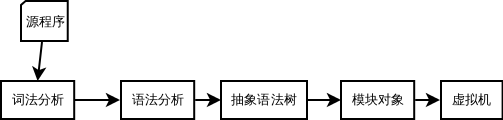
\includegraphics[scale=0.8]{file_process.png}
\label{fig:fileprocess}
\caption{解析器工作流程} 
\end{figure}



\section{词法}
codger源程序由一系列具有独立意义的基本语法单位--单词组成,单词是最小的词法单位,它们不能分割。单词分为8类:关键字,运算符,特殊符号,整数,长整数,浮点数,字符串,标识符,空白符,注释,其中空白符与注释属于无用单词,当被扫描器识别到时,会立刻被弃。

解析器中的语法识别模块用于对codger源程序进行词法分析,从输入字符流中扫描出由字符序列组成的单词。并把识别出的单词交给后面的语法分析模块进一步处理,并在识别过程中检测是否存在非法的单词。
\subsection{关键字}
codger中关键字具有专门的意义与用途,它们不能被当作一般的标识符来使用,这些关键字有:
\begin{quote}
\begin{verbatim}
and, as, attr, break, catch, class, continue, export,
do, elif, else, end, false, finally, for, from, func, 
if, import, in, inherit, new, not, or, print, private, 
protected, public, return, static, then, to, true,
try, while。
\end{verbatim}
\end{quote}
\subsection{标识符}
标识符用于定义变量,函数,类,方法等所使用的名称,解析器没有限定标识符的长度,但在定义标识符时,需要遵守一定的规则:以字母或者下画线开头,后面可以接零个或多个字母、数字、下画线,并且区会字母的大写与小写。用文法表示为:
\begin{quote}
\begin{verbatim}
identifier =(letter|"_"|)(letter|digit|"_")*
digit ="0".."9"
letter =lowercase|uppercase
lowercase ="a".."z"
uppercase ="A".."Z"
\end{verbatim}
\end{quote}
\subsection{特殊符号与运算符}
在codger中,运算符用于指定一种运算方式,特殊符号用于分隔不同的语句或者用于指定某些特定意义的用途。它们有:
\begin{quote}
\begin{verbatim}
 (   )   [   ]   .   ,  +   -   ~   *  ;
 /   %  <<   >>   <   >   <=   >=  ==  {  }
 !=   &   ^   | =   +=   -=   *=   /=  ->
 %=   &=   ^=   |=   >>=   <<=  换行符
\end{verbatim}
\end{quote}
\subsection{整数}
整数是一种与机器平台相关的数据类型,在32位机上,其表示范围为 $-2^{31}$ 到 $2^{31}-1$。而在64位机上,其表示范围为$-2^{63}$ 到 $2^{63}-1$ 。整数的表示范围有限,在设计程序时需要考虑运算结果溢出的情况。整数可以在codger源程序中显示的定义,整数又被分为二进制整数,八进制整数,十进制整数,十六进制整数。二进制整数以0b或者0B开头,后面紧接着一个或多个0或1;八进制整数以0或者0o、0O开头,后面紧接数字一个或多个0-7;十进制整数以1-9开头,后面紧接数字零个或多个0-9,或者是只有一位十进制整数0;十六进制整数以0x或都0X开头,后面紧接一个或者多个数字0-9、a-f、A-F。用文法表示为:
\begin{quote}
\begin{verbatim}
integer =decimalinteger|octinteger|hexinteger|bininteger
decimalinteger = nonzerodigit digit* | "0"
octinteger = "0" ("o" | "O") octdigit+ | "0" octdigit+
hexinteger = "0" ("x" | "X") hexdigit+
bininteger = "0" ("b" | "B") bindigit+
nonzerodigit = "1"..."9"
octdigit = "0"..."7"
bindigit = "0" | "1"
hexdigit:= digit | "a"..."f" | "A"..."F"
\end{verbatim}
\end{quote}

\subsection{长整数}
整数表示范围有限,在进行大数据运算时受到限制,Codger 提贡长整数用于解决这种问题。长整数是一种与机器无关的数据类型,可以进行任意大小的数据运算,不用去考虑数据溢出问题,但是前提是你的计算机有中够大的内存空间,来保存这些数据。 长整数可以在源程序中显示的定义,定义方法同整数一样,只有在后面多了一位字符L或者是l。用文法表示为:
\begin{quote}
 \begin{verbatim}
  longinteger = integer ("l" | "L")
 \end{verbatim}
\end{quote}

\subsection{浮点数}
在codger中采用的是32位浮点数,其数值范围约为:$-3.4*10^{-38}$ 到 $-3.4*10^{38}$ 。浮点数由三个部分组成:整数部分,浮点部分,指数部分。浮点数可以在源程序中显示定义,定义时整数部分与指数部分可以省去。用文法表示浮点数为:
\begin{quote}
 \begin{verbatim}
floatnumber = pointfloat | exponentfloat
pointfloat = [intpart] "." digit+
exponentfloat = (intpart | pointfloat) exponent
intpart = digit+
exponent = ("e" | "E") ["+" | "-"] digit+
 \end{verbatim}
\end{quote}
\subsection{字符串}
字符串可以在源程序中显示定义,使用规则为:以双引号开头和双引号结尾,中间可以是除 \verb \ 和换行符以处的任意字符,其中\verb \ 用于转义其它特殊字符,如果想要以多行的形式书写字符串,需要在每一行的未尾加上\verb \ 。用文法表示为:
\begin{quote}
 \begin{verbatim}
string =`"'stringitem*`"'
stringitem = <any source character except "\" 
				or newline or the quote> |"\"esc_item
esc_item =<any source character >
 \end{verbatim}
\end{quote}
\subsection{注释}
在Codger注释以\#号开头,直到这一行结果,解析器解析源程序,注释中的所有内容都分被忽略掉。用文法表示为:
\begin{quote}
 \begin{verbatim}
comment ="#" cm_item* newline
cm_item =<any source character except newline>
 \end{verbatim}
\end{quote}
\subsection{空白符}
Codger中的空白符由一个或都多个空格或者是制表符组成,程序中的空白符用于区分开不同的单词,或者使源程序的可读性更强。当解析器识别到空白符时,不会对它做任何的处理,只是简单的将它抛弃。用文法表示为:
\begin{quote}
 \begin{verbatim}
white_space =ws_item+
ws_item = space | tab 
 \end{verbatim}
\end{quote}


\newpage
\section{词法识别算法}
在前面一部分给出了在codger中所有的单词,以及描述单词结构的bnf文法,这些文法都是正则文法。正则文法与有限状态机具有等价性,它们之间可以相互转换\footnote{等价性的证明以及转换的方法可以参考``形式语言与自动机理论''}。而词法识别算法通常是通过构造有限状态机的方法来识别源程序中的不同类型的单词,状态机可以使用类似于lex的词法分析软件自动生成,这种方法处理起来简单,只需要遵守词法分析软件的使用规则即可,或者程序员可以通过手工来构造状态机。手工构造相比词法分析软件相比优点在于:
\begin{enumerate}
 \item 词法分析软件有固定处理框架,不能随意改变,限定了程序的灵活性。手工构造则没有这种限制。
 \item 词法分析软件根据一定算法生成有限状态机,其中有许多重复的或者是多余的状态都可以被优化掉。
\end{enumerate}
但手工构造如果处理不好,可能会随着正则语言规模的增大,复杂度也跟着增加,最终可以超出人脑可能处理的限度。下面介绍一种在codger词法分析模块中使用的一种算法--状态链。
\subsection{状态链简介}
在codger解析器的早期版本中,采用状态矩阵\footnote{大多数编译原理书本都会介绍状态矩阵算法,这里不对其进行详细说明}的方法来识别源程序中的单词。但由于状态矩阵算法会随着正则文法规模的增大,复杂度也跟着增加,每次当需要变更每个单词的结构时,都需要更改一大堆数据,使解析器的维护的扩展都变得非常困难,而且极容易出错。最后不得不放弃状态矩阵,而寻找新的方法。

状态链识别法是在codger解析器开发过程中总结出的一种非常实用和高效的算法,之所以命名为状态链,因为状态链算法处理的最多的是状态与状态之间的链接。状态链算法优点再于:
\begin{enumerate}
 \item 随着正则文法规模的变大,其复杂度一般情况下不会增加。
 \item 状态链是一种分治算法,它先通过为每一个不同类型的单词构造子状态机,然后再通过合并算法把子状态机合并在一起,合并时,不需要更改子状态机中的数据和状态,只需增加新的状态链接到子状态机中已有的状态。
 \item 状态机中的每个状态只需要处理它所接受输入事件类型,以及在该输入事件类型下的后继状态,而不用去了解状态机的整体结构。当状态机的结构发生变化时,很多状态都可以直接得到重用,使解析器的维护和扩展变得非常容易。
\end{enumerate}
\subsection{状态的结构}
状态链算法中,许多的状态链接在一起构成一个有限状态机,在每个状态中都会保存与该状态相关的基本信息,这些信息有:
\begin{enumerate}
 \item 状态是否为终态,如果是终态,同时也会保存该状态所属单词的类型,单词类型用于后面的语法分析。
 \item 字符映射数组:字符射数组长度为256,codger源程序是由字符序列组成,每当解析器从源程序中读出一个字符时,该字符的值的范围为:0到255,然后从字符映射数组获得输入事件类型。
 \item 状态能接受的输入事件类型,以及在该输入类型下所转换到的后继状态。
\end{enumerate}
用程序来描述为(attr表示属性定义):
\begin{quote}
 \begin{verbatim}
class State
    attr finally        #是否为终态
    attr token          #单词的类型
    attr input_map[256] #字符映射数组
    attr targets[]      #后继状态
end
 \end{verbatim}
\end{quote}
例如:假设状态a为不为终态,在字符`0'到`9'下转移到状态b,在`a'到`f'下转移到状态c,在其它状态下,转换到错误状态。为状态a构造状态数据为:
\begin{quote}
 \begin{verbatim}
State a
    finally=false
    token="unkown"
    input_map=[0,0,0,0,0,0,0,0,0,0,0,0,0,0,0,0
               0,0,0,0,0,0,0,0,0,0,0,0,0,0,0,0
               0,0,0,0,0,0,0,0,0,0,0,0,0,0,0,0
               1,1,1,1,1,1,1,1,1,1,0,0,0,0,0,0
               0,0,0,0,0,0,0,0,0,0,0,0,0,0,0,0
               0,0,0,0,0,0,0,0,0,0,0,0,0,0,0,0
               0,2,2,2,2,2,0,0,0,0,0,0,0,0,0,0
               0,0,0,0,0,0,0,0,0,0,0,0,0,0,0,0
                       .........
               0,0,0,0,0,0,0,0,0,0,0,0,0,0,0,0]
    targets=[err,b,c]
end  
 \end{verbatim}
\end{quote}

其中在input\_map中的省略号为112个0,状态a总共能接受三种输入事件类型,由于数组脚标从零开始,所以三种输入事件类型分别称为输入事件0,输入事件1,输入事件2
\begin{enumerate}
 \item 输人字符`0'到`9'会被映射为第1种输入事件类型,状态a在该输入类型下会转移到后继状态b,状态b保存在targets中的脚标为1的位置
 \item 输入字符`a'到`f'会被映射为第2种输入事件类型,状态a在该输入类型下会转移到后继状态c,状态c保存在targets中的脚标为2的位置
 \item 除`0'到`9'和`a'到`f'以外的所有字符会被映射到第0种输入事件类型,状态a在该输类型下会转移到后断状态err,状态err保存在targets中的脚标为0的位置。状态err是一个内置状态,用于表示源程于中单词存在错误。
\end{enumerate}

input\_map是一个256位的数组,数组元素类型为unsigned char, unsigned char占用一个字节,即一个input\_map需要256字节。但并不是每个状态都需要独自拥有一个字符映射数组。在很多情况下,许多状态的输入事件类型相似,或者是完全相同,它们可以建立一个公有的字符映射数组,用于共享,以提高内存的利用率。例如状态a在符号`c'到`z'转换到状态c,状态b在字符`a'到`f'能转换到状态c,虽然状态a与状态b能接受的输入事件类型不同,但是可能通过合并状态a与状态b输入事件,让它们共享一个字符映射数组。合并方法为:提取出字符`c'到z'与字符`a'到`f'两个序列范围的交集部分为:字符`c'到`f',即现在的有四种输入类型
\begin{quote}
1) 类型0, 字符`a'到`b' \\
2) 类型1, 字符`c'到`f' \\
3) 类型2, 字符`g'到`z' \\
4) 类型3, 除前面字符以外的所有字符。 
\end{quote}
以前状态a是在字符`c'到`z'转换到状态c,现在改为在字符`a'到`b'与字符`c' 到 `f'的情况下转换到c;以前状态b是在字符`c'到`z'转换到状态c,现在改为在字符`c'到`f'与字符`g'到`z'的情况下转移到状态c。在合并字符映射数组后,a的后继状态数组改为[c,c,err,err],b的后继状态数组为[err,c,c,err]。

Codger解析器的词法识别模块大约有90多个状态和10字符映射组成,基本上每种单词类型的所有状态共享一个状态映射数组。词法识别模块所占用的内存大约在4k左右。
\subsection{识别算法}
Codger的词法识别算法是基于有限状态机,在词法识别模块保存了一个完整的,能识别到codger语言中所有单词的有限状态机。当解析器解析codger源程序时,采用最大识别的方法,下面为识别一个单词大概步骤:
\begin{enumerate}
 \item 置当前状态置为有限状态机的开始状态
 \item 从输入字符流中读出一个字符
 \item 根据当前状态与输入字符确定下一个状态,并置当前状态为下一状态
 \item 处理当前状态,当前状态的类型有三种情况:普通状态,终态,错误状态
 \begin{enumerate}
 	\item 普通状态:跳转的步聚2
 	\item 终态:则记录下该状态与输入字符流的位置。并且跳转到步聚2
 	\item 错误状态:查看以前是否到达过终态,如果是则选择最近一次到达的终态,把多识别的字符返回给输入字符流,返回该单词的类型。如果没有到达过终态,则表明源程序中存在词法错误,返回出错信息。
 \end{enumerate}
\end{enumerate}
用代码来描述为:
\begin{quote}
\begin{verbatim}
GetToken(f)                    
    cur_state=begin_state      #设置当前状态为开始状态
    finally_state=Nil          #以及初始化程序数据
    file_pos=Nil
    while true 
        c=f.getchar()                 #从文件读出一个字符
        cur_state=cur_state.next(c)   #获取下一状态
        if cur_state==err         
            if finally_state!= Nil    #以前到达过终态
                f.set_read_pos(file_pos)  
                return finally_state.token  
            else                      #以前没有到达过终态
                return  ERR_TOKEN  
            end
        elif cur_state.finally        #如果为终态
            finally_state=cur_state   #保存该状态
            file_pos=f.get_read_pos   #保存文件的读位置
        end
    end
end 
\end{verbatim}
\begin{center}
 代码4.3.1
\end{center}
其中State.next的代码如下:
\end{quote}
\begin{quote}
\begin{verbatim}
State.next(c)
    input_type=State.input_map[c]    #获取输入类型
    return State.targets[input_type] #找到后继状态并返回
end 
\end{verbatim}
\end{quote}

涉及到识别到错误状态时,读位置的回退操作,回退的平均位移为2,所以代码4.3.1的时间算杂度与基本上与源文件的字符长度成正比。
  
\subsection{状态机的合并}
在前面介绍过,状态链算法是一种分治的算法,其主要思想为先为每个不同类型的单词构造子状态机,然后通过合并算法把子状态机合并成为一个大的综合性的状态机。假设现在有两个状态机:
\begin{quote}
1) 状态机A用于识别正则式[0-7]+abf所表示的语言,如图\ref{fig:state_a}\\
2) 状态机B用于识别正则式[4-9]+acd所表示的语言,如图\ref{fig:state_b}
\end{quote}
\begin{figure}
 \centering
 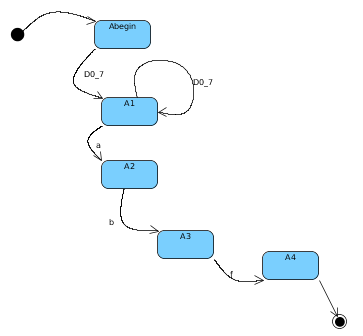
\includegraphics[scale=1]{s_a.png}
 \caption{状态机A}
 \label{fig:state_a}
\end{figure}
为了减少字符映射数组的使用,让状态机A的所有状态共享一个状态映射数组,这样一来,对于每个状态来说就有5种输入类型,同样也就有5个后继状态:
\begin{quote}
1) 数字0到7,命名为 D0\_7  \\
2) 字符a,命名为 S\_a  \\
3) 字符b,命名为 S\_b \\
4) 字符f,命名为 S\_f \\
5) 除以上字符以外的所有字符,命名为 Other
\end{quote}
例如状态机A中的状态A1的后继状态为:[A1,A2,err,err,err] 

同样对状态机B中的所有状态也让它们共享一个状态映射数组,则对于每个状态来说,输入类型有5种,5个后继状态:
\begin{quote}
1) 数字4到9,命名为 D4\_9 \\
2) 字符a,命名为 S\_a \\
3) 字符c,命名为 S\_c \\
4) 字符d, 命名为 S\_d \\
5) 除以上字符以外的所有字符,命名为 Other
\end{quote}
\begin{figure}
 \centering
 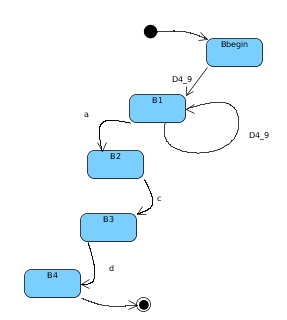
\includegraphics[scale=1]{s_b.png}
 \caption{状态机B}
 \label{fig:state_b}
\end{figure}
合并过程如下:
\begin{description}
\item[第一步:]合并状态机A与状态B的输入类型,找出相交输入类型,提取出它们的公有子集,输入类型合并的有9种:
\begin{quote}
1) 数字0到3, 命名为 D0\_3 \\
2) 数字4到7, 命名为 D4\_7 \\
3) 数字8到9, 命名为 D8\_9 \\
4) 字符a,  命名为 S\_a \\
5) 字符b,  命名为 S\_b \\
6) 字符c,  命名为 S\_c \\
7) 字符d,  命名为 S\_d \\
8) 字符f,  命名为 S\_f \\
9) 除以上字符以外的所有字符, 命名为 Other
\end{quote}
其中状态机A中的输入类型D0\_7被分解成为了输入类型D0\_3和D4\_7;状态机中的输入类型D4\_9被分解成了输入类型D4\_7和D8\_9
\item[第二步:]状态机A的开始状态为Abegin,状态机B的开始状态为Bbegin,创建一个状态复合状态 \{Abeign ,Bbegin\}, 把该复合状态命名为Cbegin,并且标记Cbegin。其中复合状态的定义为:复合状态中的任意一个状态能在某种输入类型下发生状态转移,该复合状态也能在该输入类型下发生状态转移,并且后继状态相同。
\item[第三步:]找出一个被标记的复合状态,现在只有Cbeign被标记,所以取出 Cbegin,然后取消标记 Cbeign,并确定Cbegin的后继状态,Cbeign 为 \{Abegin ,Bbegin\} 的复合状态:\\
因为:
\begin{quote}
\begin{verbatim}
f(Abegin,D0_7)->A1
f(Bbegin,D4_9)->B1
\end{verbatim}
\end{quote}
推出:
\begin{quote}
\begin{verbatim}
f(Cbegin,D0_3)->A1
f(Cbegin,D4_7)->{A1,B1}
f(Cbegin,D8_9)->B1
\end{verbatim}
\end{quote}
CBegin的转换情况如下表\footnote{空白的地方表示状态CBegin在该输入类型转移到err}:

\begin{tabular}[c]{c|c|c|c|c|c|c|c|c|c}
状态\slash输入&	D0\_3&D4\_7&D8\_9&S\_a&S\_b&S\_c&S\_d&S\_f&Other \\
\hline
CBegin&A1&A1,B1&B1&&&&&&\\
\hline
\end{tabular}

在确定后继状态,需要处理的其中的复合状态,Cbeign在输入事件D4\_7下转移到复合状\{A1,B1\},该复合状态以前并没出现过,创建复合状态\{A1,B1\},把该状态命名为C1,标记C1。
\item[第四步:] 检测现在是否存在被标记的复合状态,如果存在,跳转到第三步。如果没有,则状态机的合并完成。现在状态C1被标记,将其取出,取消标记C1,C1 为 \{A1,B1\} 的复合状态:\\
因为:
\begin{quote}
\begin{verbatim}
f(A1,D0_7)->A1
f(A1,S_a)->A2
f(B1,D4_9)->B1
f(B1,S_a)->B2
\end{verbatim}
\end{quote}
推出:
\begin{quote}
\begin{verbatim}
f(C1,D0_3)->A1
f(C1,D4_7)->{A1,B1}
f(C1,D8_9)->B1
f(C1,S_a)->{A2,B2}
\end{verbatim}
\end{quote}

C1的状态转移如下表:

\begin{tabular}[c]{c|c|c|c|c|c|c|c|c|c}
状态\slash输入&	D0\_3&D4\_7&D8\_9&S\_a&S\_b&S\_c&S\_d&S\_f&Other \\
\hline
C1&A1&A1,B1&B1&A2,B2&&&&& \\
\hline
\end{tabular}

C1的后继中状态中有两个复合状态,其中复合状态\{A1,B1\}在以前已经被创建过,所以不对其进行处理。复合状态\{A2,B2\}以前没有出现过,则创建它,并且标记,把它命名为C2。

现在还存在标记的复合状态C2,所以继续按照每二步的方法来处理,取出C2,取消标记,C2为 \{A2, B2\} 的复合状态: \\
因为:
\begin{quote}
\begin{verbatim}
f(A2,S_b)=A3
f(B2,S_c)=B3
\end{verbatim}
\end{quote}
推出:
\begin{quote}
\begin{verbatim}
f(C2,S_b)=A3
f(C2,S_c)=B3
\end{verbatim}
\end{quote}

C2的状态转移如下表:

\begin{tabular}[c]{c|c|c|c|c|c|c|c|c|c}
状态\slash输入&	D0\_3&D4\_7&D8\_9&S\_a&S\_b&S\_c&S\_d&S\_f&Other \\
\hline
C2&&&&&A3&B3&&& \\
\hline
\end{tabular}
\end{description}

现在以经没有被标记过的状态,表示状态机的整个合并过程完成,合并后创建了3个新状态:CBegin, C1, C2。每个状态接受的输入类型有9个,但可以对其进行优化,因为三个状态在输入类型 S\_d, S\_f ,Other 下都转移到err,可以把它们合并到输入类型Other中,即最终的输入类型7个:
\begin{quote}
1) 数字0到3, 命名为 D0\_3 \\
2) 数字4到7, 命名为 D4\_7 \\
3) 数字8到9, 命名为 D8\_9 \\
4) 字符a,  命名为 S\_a \\
5) 字符b,  命名为 S\_b \\
6) 字符c,  命名为 S\_c \\
7) 除以上字符以外的所有字符, 命名为 Other
\end{quote}
合并后的状态图为:图\ref{fig:state_c}, 每个状态后继状态如下:
\begin{quote}
1) CBegin后继状态为:[A1,C1,B1,err,err,err,err]  \\
2) C1后继状态为:[A1,C1,B1,C2,err,err,err] \\
3) C2后继状态为:[err,err,err,err,A3,B3,err] 
\end{quote}
\begin{figure}
\centering
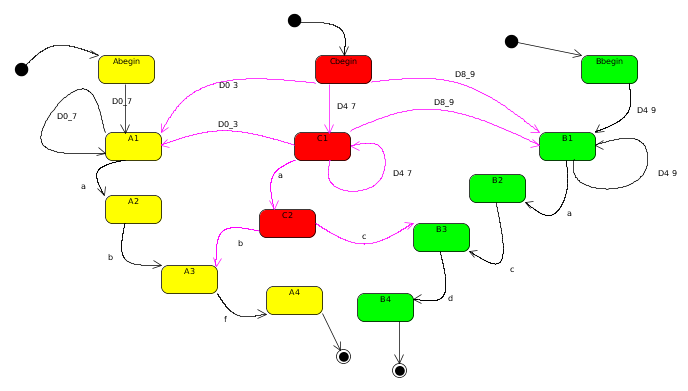
\includegraphics[scale=0.8,angle=90]{s_c.png}
\caption{状态机A与状态机B后并后}
\label{fig:state_c}
\end{figure}
状态机A与状态B的合并过程中,并不会改变状态A与状态机B的任何一个状态的信息,合并后创建了3个的新状态。新状态通过后继状态链接到子状态机A与子状态机B中的状态。把识别算法中的开始状态改为Cbegin,就可以对正则式[0-7]+abf和[4-9]+acd表示的语言进行识别。因为子状态的数据没有被改变,当只需要识别正则式[0-7]+abf所表示的语言时,同样也只需要把识别算法中的开始状态改变Abegin即可,这种特性使模块的调试变得很简单,可以先测试子状态机A和子状态机B是否正确,然后再测试合并后的状态机是否正确。

在Codger词法中有9个不同类型的单词,关键字的识别是通用先识别出标识符,然后再判断标识符是否属于关键字。子状态机有8个,识别每种单词类型子状态机的开始符号所接受的输入事件类型之间的交集很少,例如:注释以\#号开头,整数和以数字开头,浮点数以数字和点号开头,字符串以双引号开头,标识符以字母开头,在合并的时,涉及到的复合状态很少,最复杂的合并属于浮点数与整数的合并,但合并后也只创建了4个新的状态。


\section{数据类型}
\subsection{对象}
Codger语言的整体的设计思想为:一切皆是对象。整数,浮点数,字符串等基本的数据类型是对象,函数是对象,甚至类也是对象\ldots{} 因为这种特性,可以在源程序中使用类似于下面的语句:
\begin{quote}
\begin{verbatim}
print 1.add(3)  #输出1+3的值
print "Codger".length() #输出字符串"Codger"的长度
\end{verbatim}
\end{quote}
对象Object是所有对象的父类,也就是说所有对象直接或者间接的继承对象Object。每个对象所携带的信息分为两部分:1)对象的类型信息,用于标识该对象的类型,所有同类型的对象共享对象的类型信息,类型信息里面保存了对象的所属类型,对象使用私有数据的方法,对象与其它对象交互的方式等。类型信息在对象创建时绑定到对象上。2)对象的私有数据,不同的对象有不同的私有数据,不同类型的对象对私有数据的使用方法也不同,例如整数对象的私有数据部分用于保存数值,字符串对象的私有数据用于保存字符序列。
\subsection{变量}
Codger是一门动态类型语言,所有对象的类型都是在运行时才能确定,变量在使用时不需要预先申明,也不需要申明变量的类型,可以不同的时刻给变量赋值不同类型的对象,例如下面的语句:
\begin{quote}
\begin{verbatim}
a=2          #把整数对象2赋值给变量a
a="Codger"   #把字符串对象"Codger"赋值变量a 
\end{verbatim}
\end{quote}
当对一个变量赋值时,变量中会保存到该对象的引用,如果访问一个未引用对象的变量时,虚拟机会抛出变量未定义的异常。当把一个变量赋值给另一个变量,两个变量所引用的对象为同一个,例如:
\begin{quote}
\begin{verbatim}
a=[3,4]       #变量a引用一个数组对象
b=a           #把变量a赋值给变量b
a.push(5)     #调用a引用数组对象的push方法
print b       #输出b,结果为 [3,4,5]
\end{verbatim}
\end{quote}
\subsection{基本数据类型}
codegr现在支持8种基本数据类型:布尔值,整数,长整数,浮点数,字符串,数组,散列表,以及特殊类型Nil用于表示空对象,它们都可以在程序中显示定义。布尔值,整数,长整数,以及浮点数四种类型属于标量类型,一旦标量类型的对象被创建,在其生命周期内,对象的状态不会发生改变,其中:
\begin{enumerate}
\item 布尔值用于逻辑运算,也被称为逻辑值,它的值有两个,分别为真和假,假用`false'表示,真用`true'表示;
\item 整数,浮点数,长整数,用于数值运算\footnote{它们3个以及字符串的定义规则见词法部分};
\item 字符串是由多个字符组成的有限序列;
\end{enumerate}

另一种为可变类型,可变类型的对象被创建后,状态可能发生多次改变,数组和散列表属于可变类型。其中:
\begin{enumerate}
\item 数组是一种顺序性的容器,用于存储对象,定义规则为:
\begin{quote}
\begin{verbatim}
"[" [expr] { "," expr} [","] "]"
\end{verbatim}
\end{quote}
\item 散列表则是一种关联性容器,散列表中每个元素由键和值组成,键用于索引,值用于保存数据,定义规则为:
\begin{quote}
\begin{verbatim}
"{" [ expr "->" expr ] { "," expr "->" expr } [","] "}"
\end{verbatim}
\end{quote}
\end{enumerate}
定义规则使用EBNF\footnote{EBNF的全称为:Extended Backus-Naur Form,后面涉及到的文法全部都为EBNF文法}文法表示,expr表示表达式,双引号中表示字符序列, [\ldots{}]表示可选,\{\ldots{}\}表示重复零次或多次。

特殊类型Nil用于表示空对象,类似于java中的NULL对象或者是python中的None对象,在源程序中用`Nil'来访问。

\subsection{函数与匿名函数}
在Codger中一切皆为对象,函数也不例外。函数可以赋值给一个变量或者是保存在容器中,在解析器解析源程序,函数对象并不会被创建,这一点可能和其它动态语言差别很大,只有虚拟机运行到定义函数的字节码时,函数对象才被创建,同时把函数对象保存在定义函数名称同名的变量中,函数对象创建后,可以通过变量访问函数对象。如果在函数定义时,函数的名称没有指定,则该函数被视为匿名函数,匿名函数和函数属于同一种对象类型。
\subsubsection{函数创建}
每当函数对象创建时,会对当前作用域引用,当前作用域退出时,但不会被立即销毁,只有所有引用该作用域的函数对象毁销时,该作用域才会被毁销。只要函数对象存活,函数对象所在的作用域中的所有变量都被保存了下来,形成词法闭包\footnote{词法闭包:引用了自由变量的函数。这个被引用的自由变量将和这个函数一同存在,即使已经离开了创造它的环境也不例外}。如果某个函数对象所在作用域只被该函数对象引用,那么该作用域就可被视为该函数对象的私用数据空间。
\subsubsection{函数调用}
当函数对象被调用时,会创建一个新的作用域,新作用域的上层作用域会被设置为函数对象所在的作用域。多次调用函数对象,会创建多个作用域,保证了函数调用时内部变量的独立性。在Codger中变量的访问只会在当前作用域用查找,并不会查找上层作用域。在变量前面加上\$表示查找上层到顶层作用域中的变量,变量的赋值也是一样。

如果一个函数对象直接或者间接调用自身,则被称递归调用,但对于动态语言来说,递归调用的代价很高,在递归过程中的临时变量会累积起来而得不到释放,如果递归深度过大,会消耗掉很大一块的内存,同时也加大了垃圾回收例程的负担。当递归算法可以使用等价的迭代算法实现时,优先选择迭代算法。
\subsubsection{函数定义}
在Codger中使用下面的语法定义函数:
\begin{quote}
\begin{verbatim}
"func" [identifier] "(" [arg] { "," arg } [","] ")"
        stmts
"end"
\end{verbatim}
\end{quote}
其中identifier为标识符,表示函数名,当函数名为空时,则为匿名函数。arg表示函数的参数类型,参数类型有3种:
\begin{description}
\item[简单参数:]只由参数名组成,当函数调用时,参数的个数比须与定义中简单参数的个数相匹配。例如:
\begin{quote}
\begin{verbatim}
func add(x,y)
    return x+y
end 
print add(3,5)   #输出结果为 8
\end{verbatim}
\end{quote}

\item[缺省参数:]由参数名和表达式组成:\verb|identifier "=" expr|,缺省参数必须位于简单参数的后面,当函数调用时,参数个数比须大于等于简单参数的个数,参数的个数的最大值不能超过简单参数与缺省参数的总和,如果在调用时,缺省参数部分的值没有被指定,则会传入其相对应的\verb|expr|的值。例如:
\begin{quote}
\begin{verbatim}
func add_default(x,y=10)
    return x+y
end 
print add_default(1)     #输出结果为11
print add_default(1,20)  #输出结果为21
\end{verbatim}
\end{quote}
\item[多参数:]在参数名前面加上*,表示接受多个参数,多参数只能出现在参数定义的最后面,并且最多只能定义一个。当函数调用时,多参数会以数组的形式传入。例如:
\begin{quote}
\begin{verbatim}
func add_many(*x)
    sum=0
    for i in x            #遍边数组中的每一个元素
        sum+=i
    end
    return sum
end
print add_many()          #输出为0
print add_many(1,2)       #输出为3
print add_many(1,2,3,4)   #输出为10
\end{verbatim}
\end{quote}
\end{description}
如果在函数定义时,没有return语句,则返回对象Nil
\subsection{类与实例}
类是面向对象编程中基本的概念,类可以看做是有一个模板,这个模板决定了创建实例\footnote{为了和对象相区别,所以采用实例这个术语}的模样。类对象通过类似于函数调用的方法来创建实例,每个实例拥有属性和方法,实例的属性和方法统称为实例的成员。

类可以在源程序中通过关键字class定义,同函数一样,类对象的创建是在运行时,而不是在解析源程序完成时。Codger中类也被视为对象,类可以拥有自己的属性和方法。
\subsubsection{访问权限}
在Codger中访问权限是从对象的角度来设计的,每个对象拥有0个或多个成员,当某个对象想要访问其它对象的某个成员时,要确保有足够的权限,否则虚拟机在运符时会抛出访问权限异常。Codger中对象成员的访问权限分为以下三类:
\begin{enumerate}
\item 私有的:该成员只有对象自身可以访问或者赋值。
\item 受保护的:对象自身可以访问或者赋值该成员,其它对象只能访问,不能赋值。这一点和其它的面向对象编程语言例如C++或者java对受保护成员的定义差别很大。
\item 公开的:对象自身可以访问或者赋值该成员,其它对象同样也可以访问和赋值。
\end{enumerate}

\subsubsection{继承}
类可以看做是有一个模板,这个模板决定了创建实例的模样,如果另外一个类想要使用,修改或者是扩展这个模板,那么另一个类就需要继承该类。被继承的类称为父类,继承类称为子类,在源程序中可以通过关建字inherit实现。Codger中只支持单继承,一个类只能继承一个父类。继承时,父类的模板会被导入到子类的模块中,这个过程称为使用,如果在子类中,对父类模板中的某个成员重新进行了定义,则称作为修改,子类中定义父类模板中不存在的成员时,称作为父类模板的扩展。

因为Codger的访问权限是从对象的角度设计的,所以在继承过程时,权限没有任何意义,即使有在父类模板中定义为私有的成员,也会被导入到子类模板中。并且子类可以对它的模块进行任意的修改,或者是重定义模板成员中的访问权限。

\subsubsection{类定义}
在Codger中使用下面的方法来定义一个类:
\begin{quote}
\begin{verbatim}
"class" identifier [inherit expr]
    {class_stmt}
"end"

class_stmt = [perm] [static] ( attr_declare |func_declare)
attr_declare =  "attr" identifier ["=" expr] 
perm ="public" | "protected" | "private"
\end{verbatim}
\end{quote}
其中func\_declare见上一节中函数的定义, 在成员申明时如果没有指定访问权限,那么该成员的访问权限为缺省值受保护的,其中关键字static表示该成员属于类对象。在属性申明时,可以给该属性赋一个默认值,每当类创建一个实例时,实例的该属性会被设置为相应默认值。

如果在类定义实现方法init,则在类创建实例时,init方法会被调用,用于初始化实例数据,init方法也称为构造函数。

\subsection{模块} 
模块是Codger组织源文件的一个基本方式,每个源文件被加载完成时,虚拟机内部会生成一个模块对象用于表示该源文件。当一个模块需要使用其它模块的数据时,可使用import关键字将其它模块导入到当前模块。虚拟机运行到import指令时,会首先检测需要导入的模块是否被加载,如果加载,则直接导入,如果需要导入的模块还没有被加载,虚拟机会加载该模块,然后再将该模块导入。

模块可以使用export关键字,将对象导出,供其它模块访问。假设模块A导入了模块B,但模块A只能访问模块B中被导出的对象,例如:
\begin{quote}
\begin{verbatim}
---------file b.gr ------------
func add(x,y) return x+y end      #定义函数add
export add                        #导出函数add
func minus(x,y) return x-y end    #定义函数minus,但并未导出

----------file a.gr -----------
import b              #导入模块b
print b.add(1,2)      #调用模块b中的add函数,输出为3
print b.minus(2,1)    #虚拟机抛出成员minus在模块b中未定义异常

\end{verbatim}
\end{quote}







\section{运算符与表达式}
表达式\footnote{表达式的完整EBNF文法请参考附录2}是由运算符将运算对象连接起来具有合法语义的式子,运算符分为这么三类:一元运算符,后缀运算符,二元运算符。不同类型的对象对于运算符的处理方式不同,对于运算符的处理方法保存在对象的类型信息里面,例如当二元运算符+的左右操作数都为字符串对象时,返回结果为连接后的字符串;当操作数为左右整数对象时,返回结果为两个数的和。

\subsection{一元运算符}
一元运算符也称为前缀运算符,有这么4个:\begin{textbf}+, -, \verb|~|, not\end{textbf}
\begin{enumerate}
\item 运算符\textbf{ not} 用于逻辑运算,表示逻辑非;
\item 运算符\textbf{ +} 在数值运算中,表示负号。
\item 运算符\textbf{ -} 在数值运算中,表示正号。
\item 运算符\verb| ~| 在数值运算中,表示按位取反
\end{enumerate}
\subsection{后缀运算符}
在Codger后缀运算符有\textbf{ [ ] , . , ( ) } 这么3个
\begin{enumerate}
\item 运算符\textbf{[ ]},也被称为下标运算符的使用方法为:
\begin{quote}
\begin{verbatim}
expr1 "[" expr2 "]"
\end{verbatim}
\end{quote}
\begin{itemize}
\item 当expr1为字符串对象时,表示下标访问,返回结果为一个新的字符串,该字符串的内容为位于 expr1 对象的expr2位置的字符。
\item 当expr1为数组对象时,表示下标访问,返回结果为存储在 expr1 对象的expr2位置的对象。
\item 当expr1为散列表对象时,表示查询,返回结果为存储在expr1对象中健值expr2所关联的对象。
\end{itemize}
\item 运算符 \textbf{ . } 用于访问对象的属性,所以也被称为属性访问运算符,使用方法为:
\begin{quote}
\begin{verbatim}
expr "." identifier 
\end{verbatim}
\end{quote}
其中identifier为标识符,表示访问对象expr的identifier属性。
\item 运算符 \textbf{ ( ) } 用于过程调用,使用方法为:
\begin{quote}
\begin{verbatim}
expr "(" [ expr ] {"," expr} [","] ")"
\end{verbatim}
\end{quote}
当expr为函数对象时,则发生过程调用;当expr为类对象时,则会创建一个实例对象。
\end{enumerate}
\subsection{二元运算符}
 Codger中的二元运算符有18个,分别为:
\begin{quote}
\begin{verbatim}
+  -  *  /  %  
<<  >>  &  ^  |  
<  <=  ==  !=  >=  > 
and  or 
\end{verbatim}
\end{quote}
这18个运算符又被分为4类:
\begin{enumerate}
\item 算术运算符:
\begin{quote}
\begin{verbatim}
+  -  *  /  %  
\end{verbatim}
\end{quote}
在数值运算中,运算符 + 用于求和;,- 用于求差,* 用于求乘积; / 用于求商; \% 用于取模。
\item 位运算符:
\begin{quote}
\begin{verbatim}
<<  >>  &  ^  |  
\end{verbatim}
\end{quote}
在数值运算中,运算符 \verb << {} 表示左移运算,\verb >> {} 表示右移运算, \verb & {} 表示按位与运算, \verb ^ {} 表示按位异或运算,\verb | {} 表示按位或运算
\item 比较运算符:
\begin{quote}
\begin{verbatim}
<  <=  ==  !=  >=  > 
\end{verbatim}
\end{quote}
在数值运算中,运算符 \verb < {} 表示小于运算,\verb <= {} 表示小于或等于运算, \verb == {} 表示等于运算,\verb != {} 表示不等于运算,\verb >= {} 表示大于或等于运算, \verb > {} 表示大于运算。
\item 逻辑运算符:
\begin{quote}
\begin{verbatim}
and  or 
\end{verbatim}
\end{quote}
运算符and表示逻辑与运算,如果左边表达式返回的左操作数为假,则立刻返回假,而不会对右边表达进行运算;运算符or表示逻辑或运算,如果左边表达式返回的结果右操作数为真,则立刻返回真,而不会对右边表达式进行运算。逻辑运算中,当操作数不为布尔值,会进行布尔转换:整数,浮点数,长整数为0时为假,其它情况为真;数组与散列表中的元素个数为0时,为假,其它情况为真;字符串为空串时为假,其它情况为真;特殊类型Nil为假
\end{enumerate}

\subsection{类型转换}
在数值运算中,二元运算符的左右操作数为不同的数据类型时,会涉及到类型的转换,转换的优先级为:浮点数 \verb > {} 长整数 \verb > {} 整数 \verb > {} 布尔值,当转换优先级高的数据类型与转换优先级低的数据类型运算时,转换优先级低的数据类型会转换到优先级高的数据类型。

\subsection{运算符优先级}
表达式由多个运算符组成,合个运算之间的优先级别关系以及同级别运算符的运算顺序(结合方向)如下表: 
\begin{center}
\begin{tabular}{c|c|c|c}
优先级别&运算符&运算形式&结合方向 \\
\hline
&( )&(e)& \\
1&[ ]&a[e]& 从左至右 \\
& . & a.x& \\
\hline
2&+ - \verb|~| &+a&从右至左 \\
\hline
3&* / \% &e1*e2&从左至右 \\
\hline
4& + - &e1-e2&从左至右 \\
\hline 
5& \verb|<< >>| &e1 \verb|<<| e2&从左至右 \\ 
\hline
6& \verb|&| &e1 \verb|&| e2&从左至右 \\
\hline
7& \verb|^| &e1 \verb|^| e2 &从左至右 \\
\hline
8& \verb | &e1 \verb |  e2 &从左至右  \\
\hline 
9& \verb|<  <=  >  >=|& e1 \verb|<| e2 &从左至右 \\
\hline
10& \verb|==  !=| & e1 \verb|==| e2 &从左至右 \\
\hline 
11& not & not e1 & 从左至右 \\
\hline 
12& and & e1 and e2 & 从左至右 \\
\hline
13& or & e1 or e2 & 从左至右 \\
\hline
\end{tabular}
\end{center}
在表中,优先级的数值越大,其优先级越低。优先级最高的为括号,最低的为运算符 or。
\section{基本语句}
在Codger中,总共有16不同类型的语句,一个Codger源程序由一条或多条语句组成,语句与语句之间使用一个或者多个分隔符隔开,分隔符有两种:换行符和分号符。例如, 用换行符来分隔两条语句:
\begin{quote}
\begin{verbatim}
a=3
b=4
\end{verbatim}
\end{quote}
或者当需要把多条语句写到一行时,可以用分号来分隔语句,例如:
\begin{quote}
\begin{verbatim}
a=3;b=4
\end{verbatim}
\end{quote}
或者是使用类似于c风格的来分隔语句,例如:
\begin{quote}
\begin{verbatim}
a=3;
b=4; 
\end{verbatim}
\end{quote}
不同类型的语句有不同类型的语法规则,在源程只有遵守语法规则才会被解析器正确解析,Codger的语法分析模块使用bison\footnote{gnu发布的一款在linux平台下替代yacc的语法分析软件,bison完全兼容yacc}软件把描述Codger语法规则的LR(1)文法转换为LALR(1)分析表,来分析源程序的语法结构是否正确,最后生成与源程序等价的抽象语法树,以供后面的字节码生成模块进一步处理。

Codger中的16条语句被分为6类:简单语句,循环语句,选择语句,跳转语句,异常语句,定义语句,模块管理语句。下面部分依次介绍每类语句的语法规则。

\subsection{简单语句}
\subsubsection{表达式语句}
表达式在前面``表达式与算述符"这一部分已经介绍,如果一个表达式没有被其它语句使用,它的前后都有语句分隔符,在这种情况下,则被称为表达示语句,语法规则用文法表示为:
\begin{quote}
\begin{verbatim}
expr_stmt = expr 
\end{verbatim}
\end{quote}
表达式语句中,表达式会被运行,但表达式返回的结果没有其它对象引用,会被直接丢弃。\\
示例代码:
\begin{quote}
\begin{verbatim}
1+2         #计算的结果3被直丢弃
add(1+3)    #函数add返回结果4,被丢弃
\end{verbatim}
\end{quote}

\subsubsection{赋值语句}
赋值语句是给可赋值对象赋于一个值,Codger中可赋值对象有:变量,集合中的元素,对象的成员。赋值语句分为两类:1)直接赋值:将值直接赋值给可赋值对象;2)运算后再赋值:先从可赋值对象中提取出原有的值,并与将要赋的值进行指定的运算后,再赋值给可赋值对象。语法规则用文法表示为:
\begin{quote}
\begin{verbatim}
assign_stmt = assign_object assign_oper expr 
assign_oper =  "=" | "*=" | "/=" | "%=" | "+=" |
               "-=" | "<<=" | ">>=" | "&=" | "^=" | "|="
assign_object = expr
\end{verbatim}
\end{quote}
其中expr为以变量,[expr], .identifier 结尾的表达式。
示例代码:
\begin{quote}
\begin{verbatim}
a=3+4     
$a=4      
coord.x=0.3
array[3]+=4
\end{verbatim}
\end{quote}
\subsubsection{print语句}
print语句用于将对象的值输出到标准输出端,语法规则用文法表示为:
\begin{quote}
\begin{verbatim}
print_stmt =  "print" [expr] { "," expr }
\end{verbatim}
\end{quote}
示例代码:
\begin{quote}
\begin{verbatim}
print 2                    #输出:  2
print "Codger"+"Is"+"Good" #输出:  "CodgerIsGood"
print 3+3,3+4,1+2          #输出:  6 7 3
a=[3,4,5]
print a                    #输出:  [3,4,5]
\end{verbatim}
\end{quote}



\subsection{循环语句}
\subsubsection{for语句}
for语句用于遍历可迭代对象中的每一个元素,Codger中的可迭代对象有数组和散列表。语法规则用文法表示为:
\begin{quote}
\begin{verbatim}
for_stmt = "for" assign_object "in" expr for_delimiter
                stmts
            "end"
for_delimiter = "\n" | ";" | "do"
\end{verbatim}
\end{quote}
在for语句运行时,每次从expr返回对象中取出一个元素,赋值给可赋值对象 assign\_object,并执行语句stmts。当expr返回对象中的每个元素都被遍历完成时,for语句结束。\\
示例代码:
\begin{quote}
\begin{verbatim}
a=[3,4,5,5]
sum=0
for i in a
    sum+=i
end
print sum   #输出为17
\end{verbatim}
\end{quote}

\subsubsection{while语句}
while语句由一个控制表达式和子语句组成,while语句循环执行子语句中的内容,直到表达式的结果为假,语法规则文法表示为:
\begin{quote}
\begin{verbatim}
while_stmt = "while" expr while_delimiter
                  stmts
             "end"
while_delimiter = "\n" | ";" | "do"
\end{verbatim}
\end{quote}
示例代码:
\begin{quote}
\begin{verbatim}
i=0
sum=0
while i<=100
    sum+=i
    i+=1
end 
print sum  #输出为: 5050
\end{verbatim}
\end{quote}

\subsection{选择语句}
\subsubsection{if-elif-else语句}
if-elif-else语句由一个if部分,零个或多个elif部分,零个或一个else部分组成。if 和 elif 部分由控制表达式和子语句组成,else部分由一个子语句组成。if-elif-else语句运行时,先从if部分开始判断控制表达式是否为真,如果为真,则执行if部分的子语句,并退出if-elif-else语句,如果为假,则会依次判断elif的控制表达式,elif的控制表达式如果为真,则执行相对应的elif的子语句,并退出if-elif-else语句。如果elif的控制表达式为假,则判断下一个elif部分。最后如果if-elif-else还没有退出,则执行else部分的语句。语法规则用文法表示为:
\begin{quote}
\begin{verbatim}
if_stmt = if_part  {elif_part} [else_part] "end"
if_part = "if" expr if_delimiter stmts 
elif_part = "elif" expr if_delimiter stmts
else_part = "else" stmts
if_delimiter = "\n" | ";" | "then"
\end{verbatim}
\end{quote}
示例代码:
\begin{quote}
\begin{verbatim}
a=2
if a==1
    print 1
elif a==2
    print 2
else 
    print "unkown"
end 
#输出为 2
\end{verbatim}
\end{quote}

\subsection{跳转语句}
\subsubsection{break语句}
break语句用于在循环语句中,当循环语句执行时,遇到break语句,则会退出循环,语法规则用文法表示为
\begin{quote}
\begin{verbatim}
break_stmt = "break" 
\end{verbatim}
\end{quote}
示例代码:
\begin{quote}
\begin{verbatim}
a=[1,2,3,4,5,6] 
sum=0
for i in a
    if a ==3
        break
    end 
    sum+=i
end 
print sum   #输出为: 3
\end{verbatim}
\end{quote}

\subsubsection{continue语句}
continue语句用于循环语句中,当循环语句执行时,遇到continue语句,则会放弃执行当前循环后面的内容,重新开始下一次循环,语法规则使用文法表示为
\begin{quote}
\begin{verbatim}
continue_stmt = "continue" 
\end{verbatim}
\end{quote}
示例代码
\begin{quote}
\begin{verbatim} 
i=0
sum=0
while i<10
    i+=1
    if i%2==0
        continue
    end 
    sum+=i
end 
print sum   #输出为: 25
\end{verbatim}
\end{quote}

\subsubsection{return语句}
return 语句用来终止一个函数的执行,并返回表达式的值。 如果表达式被省略,或在函数内没有执行return语句,则值Nil。当执行return语句时,即使函数体中仍然还有其他语句,此函数也会停止执行。语法规则使用文法表示为:
\begin{quote}
\begin{verbatim}
return_stmt = "return" [ expr ]
\end{verbatim}
\end{quote}
示例代码:
\begin{quote}
\begin{verbatim}
func add(x,y)
    return x+y
end 

print add(3,4)   #输出为7
\end{verbatim}
\end{quote}
\subsection{异常语句}
\subsubsection{throw语句}
生成一个可由 try-catch-finally 语句处理的错误或异常,语法规则用文法表示为:
\begin{quote}
\begin{verbatim}
throw_stmt = "throw" [ expr ]
\end{verbatim}
\end{quote}
示例代码:
\begin{quote}
\begin{verbatim}
print 3
throw Error("Some Error Happend")
print 4

#输出为:  3
#         Error: "Some Error Happend"
\end{verbatim}
\end{quote}


\subsubsection{try-catch-finally语句}
try-catch-finally语句提供一种机制,用于捕捉在块的执行期间发生的各种异常。此外try-finally-catch语句还能让您指定一个代码块,并保证当控制离开try语句时,先执行该代码。语法规则用文法表示为:
\begin{quote}
\begin{verbatim}
try_stmt = ( try_part finally_part  "end") |
           ( try_part [catch_part] {catch_part} 
                      [finally_part] "end" )
try_part = "try" try_demiliter stmts
catch_part = "catch" [expr] { "," expr } ["as" identifier]
             try_demiliter stmts
finally = "finally" try_demiliter stmts
try_demiliter = "\n"|";"
\end{verbatim}
\end{quote}
示例代码:
\begin{quote}
\begin{verbatim}
try 
    i=a   #变量a未定义,运行时会抛出NameError
catch NameError as e
    print "Catch "+e.name+"Not Defined"
end 
#输出为: "Catch a Not Defined"
\end{verbatim}

\end{quote}


\subsection{定义语句}
\subsubsection{函数定义语句}
函数定义语句见``数据类型--函数''那一部分
\subsubsection{类定义语句}
类定义语句见``数据类型--类''那一部分

\subsection{模块管理语句}
模块是Codger组织源文件的一个基本方式,每个源文件被加载完成时,虚拟机内部会生成一个模块对象用于表示该源文件。
\subsubsection{import语句}
import语句用于导入其它模块到当前模块中,语法规则用文法表示为
\begin{quote}
\begin{verbatim}
import_stmt ="import" identifier 
             {"." identifier} [ "as" identifier]
\end{verbatim}
\end{quote}
示例代码:
\begin{quote}
\begin{verbatim}
import math
print math.cos(math.pi)    #输出为: -1
\end{verbatim}
\end{quote}
\subsubsection{export语句}
export用于把当前模块的对象导出,供其它模块访问,使用语法规则用文法表示为:
\begin{quote}
\begin{verbatim}
export_stmt = ( "export" identifier ) |
              ( "export" expr "as" identifier )
\end{verbatim}
\end{quote}
示例代码:
\begin{quote}
\begin{verbatim}
func add(x,y)
    return x+y
end 
export add    #当被其它模块导入时,函数add可以被其它模块访问到
\end{verbatim}
\end{quote}















\appendix
\section{字节码的内部执行过程}
\subsection{不带参数的字节码}
\begin{enumerate}
\item OP\_CALL: 方法调用,需要操作数2个,例如: cos(3) \\
执行过程为:
\begin{quote}
\begin{verbatim}
r1=dstack.pop()
r0=dstack.pop()
acc=r0.call(Nil,r1)
dstack.push(acc)
\end{verbatim}
\end{quote}

\item OP\_CALL\_WITH\_HOST: 调用对象的方法,需要操作数3个,例如:a.add(3)\\
执行过程为:
\begin{quote}
\begin{verbatim}
r2=dstack.pop()
r1=dstack.pop()
r0=dstack.pop()
acc=r1.op_call(r1,r2)
dstack.push(acc)
\end{verbatim}
\end{quote}

\item OP\_SET\_ITEM: 给集合指定的元素赋值,需要3个操用数。例如: a[3]=4  \\
执行过程为: 
\begin{quote}
\begin{verbatim}
r2=dstack.pop()
r1=dstack.pop()
r0=dstack.pop()
r1.set_item(r2,r0)
\end{verbatim}
\end{quote}

\item OP\_GET\_ITEM: 访问集合中指定的元素,需要2个操作数,例如: a[3] \\
执行过程为:
\begin{quote}
\begin{verbatim}
r1=dstack.pop()
r0=dstack.pop()
acc=r0.get_item(r1)
dstack.push(acc)
\end{verbatim}
\end{quote}

\item OP\_POSITIVE: 一元运算符 + ,需要1个操作数,例如: +a \\
执行过程为:
\begin{quote}
\begin{verbatim}
r0=dstack.pop()
acc=r0.positive()
dstack.push(acc) 
\end{verbatim}
\end{quote}

\item OP\_NEGATIVE: 一元运算符 - ,需要1个操作数,例如:-a \\
执行过程为:
\begin{quote}
\begin{verbatim}
r0=dstack.pop()
acc=r0.negative()
dstack.push(acc)
\end{verbatim}
\end{quote}

\item OP\_NEGATED: 一元运算符 \verb|~| ,需要1个操作数,例如:\verb|~|a \\
执行过程为:
\begin{quote}
\begin{verbatim}
r0=dstack.pop()
acc=r0.negated()
dstack.push(acc)
\end{verbatim}
\end{quote}

\item OP\_MUL: 二元运算符 * ,需要2个操作数,例如:1*2 \\
执行过程为:
\begin{quote}
\begin{verbatim}
r1=dstack.pop()
r0=dstack.pop()
acc=r0.mul(r1)
dstack.push(acc)
\end{verbatim}
\end{quote}

\item OP\_DIV:二元运算符 \verb|/| ,需要2个操作数,例如:1\verb|/|2 \\
执行过程为:
\begin{quote}
\begin{verbatim}
r1=dstack.pop()
r0=dstack.pop()
acc=r0.div(r1)
dstack.push(acc)
\end{verbatim}
\end{quote}

\item OP\_MOD:二元运算符 \verb|%| ,需要2个操作数,例如:1\verb|%|2 \\
执行过程为:
\begin{quote}
\begin{verbatim}
r1=dstack.pop()
r0=dstack.pop()
acc=r0.mod(r1)
dstack.push(acc)
\end{verbatim}
\end{quote}

\item OP\_PLUS:二元运算符 \verb|+| ,需要2个操作数,例如:1\verb|+|2 \\
执行过程为:
\begin{quote}
\begin{verbatim}
r1=dstack.pop()
r0=dstack.pop()
acc=r0.plus(r1)
dstack.push(acc)
\end{verbatim}
\end{quote}

\item OP\_MINUS:二元运算符 \verb|-| ,需要2个操作数,例如:1\verb|-|2 \\
执行过程为:
\begin{quote}
\begin{verbatim}
r1=dstack.pop()
r0=dstack.pop()
acc=r0.minus(r1)
dstack.push(acc)
\end{verbatim}
\end{quote}

\item OP\_LSHIFT:二元运算符 \verb|<<| ,需要2个操作数,例如:1\verb|<<|2 \\
执行过程为:
\begin{quote}
\begin{verbatim}
r1=dstack.pop()
r0=dstack.pop()
acc=r0.lshift(r1)
dstack.push(acc)
\end{verbatim}
\end{quote}

\item OP\_RSHIFT:二元运算符 \verb|>>| ,需要2个操作数,例如:1\verb|>>|2 \\
执行过程为:
\begin{quote}
\begin{verbatim}
r1=dstack.pop()
r0=dstack.pop()
acc=r0.rshift(r1)
dstack.push(acc)
\end{verbatim}
\end{quote}

\item OP\_AND:二元运算符 \verb|&| ,需要2个操作数,例如:1\verb|&|2 \\
执行过程为:
\begin{quote}
\begin{verbatim}
r1=dstack.pop()
r0=dstack.pop()
acc=r0.and(r1)
dstack.push(acc)
\end{verbatim}
\end{quote}

\item OP\_XOR:二元运算符 \verb|^| ,需要2个操作数,例如:1\verb|^|2 \\
执行过程为:
\begin{quote}
\begin{verbatim}
r1=dstack.pop()
r0=dstack.pop()
acc=r0.xor(r1)
dstack.push(acc)
\end{verbatim}
\end{quote}

\item OP\_OR:二元运算符 \verb^|^ ,需要2个操作数,例如:1\verb^|^2 \\
执行过程为:
\begin{quote}
\begin{verbatim}
r1=dstack.pop()
r0=dstack.pop()
acc=r0.or(r1)
dstack.push(acc)
\end{verbatim}
\end{quote}

\item OP\_LT:二元运算符 \verb|<| ,需要2个操作数,例如:1\verb|<|2 \\
执行过程为:
\begin{quote}
\begin{verbatim}
r1=dstack.pop()
r0=dstack.pop()
acc=r0.lt(r1)?true:false
dstack.push(acc)
\end{verbatim}
\end{quote}

\item OP\_LE:二元运算符 \verb|<=| ,需要2个操作数,例如:1\verb|<=|2 \\
执行过程为:
\begin{quote}
\begin{verbatim}
r1=dstack.pop()
r0=dstack.pop()
acc=r0.le(r1)?true:false
dstack.push(acc)
\end{verbatim}
\end{quote}

\item OP\_EQ:二元运算符 \verb|==| ,需要2个操作数,例如:1\verb|==|2 \\
执行过程为:
\begin{quote}
\begin{verbatim}
r1=dstack.pop()
r0=dstack.pop()
acc=r0.eq(r1)?true:false
dstack.push(acc)
\end{verbatim}
\end{quote}

\item OP\_NE:二元运算符 \verb|!=| ,需要2个操作数,例如:1\verb|!=|2 \\
执行过程为:
\begin{quote}
\begin{verbatim}
r1=dstack.pop()
r0=dstack.pop()
acc=r0.ne(r1)?true:false
dstack.push(acc)
\end{verbatim}
\end{quote}

\item OP\_GE:二元运算符 \verb|>=| ,需要2个操作数,例如:1\verb|>=|2 \\
执行过程为:
\begin{quote}
\begin{verbatim}
r1=dstack.pop()
r0=dstack.pop()
acc=r0.ge(r1)?true:false
dstack.push(acc)
\end{verbatim}
\end{quote}

\item OP\_GT:二元运算符 \verb|>| ,需要2个操作数,例如:1\verb|>|2 \\
执行过程为:
\begin{quote}
\begin{verbatim}
r1=dstack.pop()
r0=dstack.pop()
acc=r0.gt(r1)?true:false
dstack.push(acc)
\end{verbatim}
\end{quote}

\item OP\_BOOL:布尔类型转换,需要1个操作数\\
执行过程为:
\begin{quote}
\begin{verbatim}
r0=dstack.pop()
acc=r0.bool()
dstack.push(acc)
\end{verbatim}
\end{quote}

\item OP\_BOOL\_NOTAKE:布尔类型转换,需要1个操作数,但操作数不会被弹出数据栈\\
执行过程为:
\begin{quote}
\begin{verbatim}
r0=dstack.top()
acc=r0.bool()
dstack.push(acc)
\end{verbatim}
\end{quote}

\item OP\_LOGIC\_NOT:逻辑运算符not,需要1个操作数,例如:not 1 \\
执行过程为:
\begin{quote}
\begin{verbatim}
r0=dstack.pop()
acc=not r0.bool()
dstack.push(acc)
\end{verbatim}
\end{quote}

\item OP\_PRINT:输出指令,需要1个操作数,例如: print ``Codger'' \\
执行过程为:
\begin{quote}
\begin{verbatim}
r0=dstack.pop()
r0.print()
\end{verbatim}
\end{quote}

\item OP\_PRINT\_LN:输出换行符指令,不需操作数,例如:print \\
执行过程为:
\begin{quote}
\begin{verbatim}
print("\n")
\end{verbatim}
\end{quote}

\item OP\_ITER:获取对象的迭代器,需要1个操作数 \\
执行过程为:
\begin{quote}
\begin{verbatim}
r0=dstack.pop()
acc=r0.iter()
dstack.push(r0)
\end{verbatim}
\end{quote}

\item OP\_ITER\_NEXT:获取迭代器的下一个元素,需要1个操作数,但操作数不会被弹出数据栈 \\
执行过程为:
\begin{quote}
\begin{verbatim}
r0=dstack.top()
acc=r0.iter_next()
if acc != iter_stop
    pc+=3
    dstack.push(acc)
end
\end{verbatim}
\end{quote}

\item OP\_ARRAY\_BEGIN:创建一个数组对象,需要0个操作数 \\
执行过程为:
\begin{quote}
\begin{verbatim}
acc=Array()       #创建函数对象
dstack.push(acc)
\end{verbatim}
\end{quote}

\item OP\_ARRAY\_PUSH:向数组对象的尾部增加元素,需要2个操作数 \\
执行过程为:
\begin{quote}
\begin{verbatim}
r0=dstack.pop()
r1=dstack.pop()
r0.push_back(r1)
dstack.push(r0)
\end{verbatim}
\end{quote}

\item OP\_ARRAY\_END:保留指令
\item OP\_FUNC\_BEGIN:创建一个函数对象,需要0个操作数 \\
执行过程为:
\begin{quote}
\begin{verbatim}
acc=Func()                 #创建函数对象
acc.set_scope(cur_scope)   #引用当前作用域
dstack.push(acc)
\end{verbatim}
\end{quote}

\item OP\_FUNC\_DEFAULT\_ARGS:设置函数对象的默认参数的值,如果函数有多个默认参数,该指令会把值赋给第一个还未设置的默认参数,需要2个操作数 \\
执行过程为:
\begin{quote}
\begin{verbatim}
r1=dstack.pop()
r0=dstack.pop()
r0.set_defalut_arg(r1)
dstack.push(r0)
\end{verbatim}
\end{quote}

\item OP\_CLASS\_INHERIT:类对象继承另一个类对象,需要操作数2个 \\
执行过程为:
\begin{quote}
\begin{verbatim}
r1=dstack.pop()
r0=dstack.pop()
r0.set_inherit(r1)
dstack.push(r0)
\end{verbatim}
\end{quote}

\item OP\_LOAD\_NIL:把空对象Nil压入数据栈,需要0个操作数  \\
执行过程为:
\begin{quote}
\begin{verbatim}
acc=Nil
dstack.push(acc)
\end{verbatim}
\end{quote}

\item OP\_DISCARD:从数据栈中弹出一个对象,并抛弃,需要0个操作数 \\
执行过程为:
\begin{quote}
\begin{verbatim}
dstack.pop()
\end{verbatim}
\end{quote}

\item OP\_DUP\_DATA1:复制数据栈栈顶的对象,需要0个操作数 \\
执行过程为:
\begin{quote}
\begin{verbatim}
r0=dstack.top()
dstack.push(r0)
\end{verbatim}
\end{quote}

\item OP\_DUP\_DATA2:复制数据栈栈顶的2个对象,需要0个操作数 \\
执行过程为:
\begin{quote}
\begin{verbatim}
r2=dstack[sp-1]
r1=dstack[sp-2]
dstack.push(r0)
dstack.push(r1)
\end{verbatim}
\end{quote}

\item OP\_DUP\_DATA3:复制数据栈栈顶的3个对象,需要0个操作数 \\
执行过程为:
\begin{quote}
\begin{verbatim}
r2=dstack[sp-1]
r1=dstack[sp-2]
r0=dstack[sp-3]
dstack.push(r0)
dstack.push(r1)
dstack.push(r2)
\end{verbatim}
\end{quote}

\item OP\_DATA\_SWAP0\_1:交换数据栈栈顶第0个对象与第1个对象,需要0个操作数 \\
执行过程为:
\begin{quote}
\begin{verbatim}
acc=dstack[sp-1]
dstack[sp-1]=dstack[sp-2]
dstack[sp-2]=acc
\end{verbatim}
\end{quote}

\item OP\_DATA\_SWAP0\_2:交换数据栈栈顶第0个对象与第2个对象,需要0个操作数 \\
执行过程为:
\begin{quote}
\begin{verbatim}
acc=dstack[sp-1]
dstack[sp-1]=dstack[sp-3]
dstack[sp-3]=acc
\end{verbatim}
\end{quote}

\item OP\_DATA\_SWAP0\_3:交换数据栈栈顶第0个对象与第3个对象,需要0个操作数 \\
执行过程为:
\begin{quote}
\begin{verbatim}
acc=dstack[sp-1]
dstack[sp-1]=dstack[sp-4]
dstack[sp-4]=acc
\end{verbatim}
\end{quote}

\item OP\_EXIT:退出指令,需要0个操作数 \\
执行过程为:
\begin{quote}
\begin{verbatim}
EgThread.exit()
\end{verbatim}
\end{quote}

\item OP\_RETURN:栈帧返回指令,需要1个操作数 \\
执行过程为:
\begin{quote}
\begin{verbatim}
r0=dstack.pop()
EgThread.return(r0)
\end{verbatim}
\end{quote}

\item OP\_RETURN\_NIL:栈帧返回指令,需要0个操作数 \\
执行过程为:
\begin{quote}
\begin{verbatim}
r0=Nil
EgThread.return(r0)
\end{verbatim}
\end{quote}
\end{enumerate}




\subsection{带参数的字节码}
\begin{enumerate}
\item OP\_GET\_ATTR:访问对象成员,需要1个操作数 \\
执行过程为:
\begin{quote}
\begin{verbatim}
r0=dstack.pop()
r1=symbols_pool[rd]
acc=r0.get_attr(r1,r0==sframe.host)
dstack.push(acc)
\end{verbatim}
\end{quote}
其中sframe表示当前的栈帧,host为sframe的属主对象,rd是指令的参数。

\item OP\_SET\_ATTR:给对象的成员赋值,需要2个操作数 \\
执行过程为:
\begin{quote}
\begin{verbatim}
r0=dstack.pop()
r1=dstack.pop()
r2=symbols_pool[rd]
r1.set_attr(r2,r0,r1==sframe.host)
\end{verbatim}
\end{quote}

\item OP\_CLASS\_BEGIN:创建一个类对象,需要0个操作数 \\
执行过程为:
\begin{quote}
\begin{verbatim}
acc=Class()
r0=symbols_pool[rd]
acc.set_name(r0)
dstack.push(acc)
\end{verbatim}
\end{quote}

\item OP\_CLASS\_TEMPLATE:向类的模板中增加元素,需要2个操作数 \\
执行过程为:
\begin{quote}
\begin{verbatim}
r2=perm_symbols_pool[rd]
r1=dstack.pop()
r0=dstack.pop()
r0.add_template(r2,r1)
dstack.push(r0)
\end{verbatim}
\end{quote}

\item OP\_CLASS\_ATTR:设置类对象的属性或方法,需要2个操作数 \\
执行过程为:
\begin{quote}
\begin{verbatim}
r2=perm_symbols_pool[rd]
r1=dstack.pop()
r0=dstack.pop()
r0.set_attr(r2,r1)
dstack.push(r0)
\end{verbatim}
\end{quote}

\item OP\_FUNC\_OPCODE:设置函数对象的字节码,需要1个操作数,但不会弹出数据栈 \\
执行过程为:
\begin{quote}
\begin{verbatim}
r0=dstack.top()
r1=opcodes_pool[rd]
r0.set_opcode(r1)
\end{verbatim}
\end{quote}

\item OP\_LOAD\_CONST:加载常量到数据栈,需要0个操作数 \\
执行过程为:
\begin{quote}
\begin{verbatim}
acc=consts_pool[rd]
dstack.push(acc)
\end{verbatim}
\end{quote}

\item OP\_LOAD\_SYMBOL:从当前作用域中查找符号的值到数据栈,需要0个操作数 \\
执行过程为:
\begin{quote}
\begin{verbatim}
r0=symbols_pool[rd]
acc=scope.lookup(r0)
dstack.push(acc)
\end{verbatim}
\end{quote}

\item OP\_LOAD\_U\_SYMBOL:从上层作用域到顶层作用域中查找符号的值到数据栈,需要0个操作数 \\
执行过程为:
\begin{quote}
\begin{verbatim}
r0=symbols_pool[rd]
acc=scope.lookup_upper(r0)
dstack.push(acc)
\end{verbatim}
\end{quote}

\item OP\_STORE\_SYMBOL:把符号的值到存入到当前作用域,需要1个操作数 \\
执行过程为:
\begin{quote}
\begin{verbatim}
r0=dstack.pop()
r1=symbols_pool[rd]
scope.map(r1,r0)
\end{verbatim}
\end{quote}

\item OP\_STORE\_U\_SYMBOL:把符号的值到存入到上层作用域,需要1个操作数 \\
执行过程为:
\begin{quote}
\begin{verbatim}
r0=dstack.pop()
r1=symbols_pool[rd]
scope.map_upper(r1,r0)
\end{verbatim}
\end{quote}

\item OP\_IMPORT:模块导入指令,需要0个操作数 \\
执行过程为:
\begin{quote}
\begin{verbatim}
r0=symbols_pool[rd]
acc=EgThread.import(r0)
dstack.push(acc)
\end{verbatim}
\end{quote}

\item OP\_EXPORT:导出指令,需要1个操作数 \\
执行过程为:
\begin{quote}
\begin{verbatim}
r0=dstack.pop()
r1=symbols_pool[rd]
cur_module.set_attr(r1,r0)
\end{verbatim}
\end{quote}

\item OP\_BREAK:保留指令,用于辅助字节码生成,最终会被 OP\_JUMPR* 指令代替。
\item OP\_CONTINUE:保留指令,用于辅助字节码生成,最终会被 OP\_JUMPR* 指令代替。

\item OP\_JUMPR\_FORWARD:向前跳转指令,需要0个操作数 \\
执行过程为:
\begin{quote}
\begin{verbatim}
pc+=rd-3
\end{verbatim}
\end{quote}

\item OP\_JUMPR\_BACK:向后跳转指令,需要0个操作数 \\
执行过程为:
\begin{quote}
\begin{verbatim}
pc-=rd+3
\end{verbatim}
\end{quote}

\item OP\_JUMPR\_FALSE\_FORWARD:向前跳转指令,只有假时执行,需要1个操作数 \\
执行过程为:
\begin{quote}
\begin{verbatim}
r0=dstack.pop()
rs=r0.bool()
if(not rs) pc+=rd-3
\end{verbatim}
\end{quote}

\item OP\_JUMPR\_TRUE\_FORWARD:向前跳转指令,只有真时执行,需要1个操作数 \\
执行过程为:
\begin{quote}
\begin{verbatim}
r0=dstack.pop()
rs=r0.bool()
if(rs) pc+=rd-3
\end{verbatim}
\end{quote}

\item OP\_JUMPR\_FALSE\_BACK:向后跳转指令,只有假时执行,需要1个操作数 \\
执行过程为:
\begin{quote}
\begin{verbatim}
r0=dstack.pop()
rs=r0.bool()
if(not rs) pc-=rd+3
\end{verbatim}
\end{quote}

\item OP\_JUMPR\_TRUE\_BACK:向后跳转指令,只有真时执行,需要1个操作数 \\
执行过程为:
\begin{quote}
\begin{verbatim}
r0=dstack.pop()
rs=r0.bool()
if(rs) pc-=rd+3
\end{verbatim}
\end{quote}
\end{enumerate}

\end{CJK}
\end{document}
